% This document provides the style to be used for a MSc Thesis at the
% Parallel and Distributed Systems group
\documentclass[11pt,twoside,a4paper,openright]{report}

% math packages
\usepackage{amsmath}
\usepackage{amssymb}
\usepackage{mathtools}
\usepackage{amsthm}

% textblocks for title page
\usepackage[absolute]{textpos}

% use babel for proper hyphenation
\usepackage[british]{babel}

% Graphics: different for pdflatex or dvi output, choose one
%%\usepackage[dvips]{graphicx}
%%\usepackage[pdftex]{graphicx}
\usepackage{graphicx}

\usepackage{epstopdf}
\usepackage{rotating}
\usepackage{subfigure}

% FONT
\usepackage[scaled=.92]{helvet}
%\usepackage{times}

% for url's use "\url{http://www.google.com/}"
\usepackage{url}
\usepackage[plainpages=false]{hyperref} 
\usepackage{cleveref}



\usepackage{enumitem}

\usepackage[colorinlistoftodos,prependcaption,textsize=tiny]{todonotes}


\usepackage{pifont}% http://ctan.org/pkg/pifont
\newcommand{\cmark}{\ding{51}}%
\newcommand{\xmark}{\ding{55}}%















\usepackage{tikz}
\usetikzlibrary{positioning,arrows}

\tikzset{
  block/.style={
    draw,
    rectangle,
    minimum height=1cm,
    minimum width=1cm,
    align=center
  },
  subblock/.style={
    draw,
    rectangle,
    minimum height=.75cm,
    minimum width=1.5cm,
    align=center
  },
  line/.style={->,>=latex},
  XOR/.style={draw,circle,append after command={
        [shorten >=\pgflinewidth, shorten <=\pgflinewidth,]
        (\tikzlastnode.north) edge (\tikzlastnode.south)
        (\tikzlastnode.east) edge (\tikzlastnode.west)
        }
    },
    LED/.style={draw,circle,append after command={
        [shorten >=\pgflinewidth, shorten <=\pgflinewidth,]
        %(\tikzlastnode.north) edge (\tikzlastnode.south)
        %(\tikzlastnode.east) edge (\tikzlastnode.west)
        }
    },
  dot/.style={draw,circle,minimum size=2mm,inner sep=0pt,outer sep=0pt,fill=black},
}




















% Information that will be filled in at various points in the report
\newcommand{\reportTitle}{Leveraging VLC for energy disaggregation in Smart Buildings}
\newcommand{\reportAuthor}{Johnny Verhoeff}
\newcommand{\reportEmail}{j.s.c.j.verhoeff@student.tudelft.nl}
\newcommand{\reportUrlEmail}{\href{mailto:\reportEmail}{\reportEmail}}
\newcommand{\reportMSC}{Embedded Systems} %{Embedded Systems}{Computer Engineering}{Computer Science}{Electrical Engineering}
\newcommand{\reportDate}{\today} %TODO: Dit is de datum van uitgifte van final versie aan de afstudeer commissie 
\newcommand{\presentationDate}{24th October 2016} %TODO: Dit is de datum van de afstudeerpresentatie 
\newcommand{\graduationCommittee}{

Chair: Prof. dr. K.G. Langendoen, Faculty EEMCS, TU Delft \\
Committee member: dr. ir. L.M. Ramirez Elizondo, Faculty DCE\&S, TU Delft \\ 
Committee member: dr. ir. M.A. Z\'u\~niga Zamalloa, Faculty EEMCS, TU Delft \\


} 

\newcommand{\reportAbstract}{
  
Energy consumption is an ever pressing issue.
Therefor it is needed to know what that energy is being used for.
Smart-meters can already disaggregate home appliances by looking at the distinct energy signatures of appliances.
But other items such as lighting has not been successful yet in disaggregating on a per lamp basis, due to the similar energy signatures lighting has.
In this work IDs are assigned to lights which are transmitted by the light via VLC.
The modulation of the ID will also propagate through the current that the lights draw.
To this purpose coding sequences were investigated that would allow for disaggregation of these lights by looking at the aggregated energy use, so that individual lights can be identified as being on or off.
With piggybacking on VLC, each light will get a unique ID, that they can transmit via VLC and the same ID will also be transmitted through the power they draw due to the modulation.
Hardware was designed, specifically to let that ID map into the energy signature.
And experiments were performed with commercial LEDs.
With a setup of multiple LEDs, each LED could be successfully identified as being on or off, in both DC and AC environments.
Furthermore, simulations have been performed in order to show the scalability of the proposed method.
And multiple items are highlighted that could be improved or otherwise investigated.













}
%\newcommand{\reportKeywords}{TODO KEYWORDS}

% For pdflatex
\pdfinfo{
   /Author (\reportAuthor)
   /Title  (\reportTitle)
   %/Keywords (\reportKeywords)
}

\begin{document}

\pagenumbering{alph}
\pagestyle{empty}





\renewcommand*{\chapterautorefname}{Chapter}




% FRONTCOVER
\include{template/frontcover}

%%%%%%%%%%%%%%%%%%%%%%%%%%%%%%%%%%%%%%%%%%%%%%%%%%%%%%%%%%%%%%%%%%%%%%%%%%%%%%%
\hoffset=1.63cm
\oddsidemargin=0in
\evensidemargin=0in
\textwidth=5in

%%%%%%%%%%%%%%%%%%%%%%%%%%%%%%%%%%%%%%%%%%%%%%%%%%%%%%%%%%%%%%%%%%%%%%%%%%%%%%%
\parindent=1em

% EMPTY PAGE
\cleardoublepage

\pagestyle{plain}
\pagenumbering{roman}
\setcounter{page}{1}

% TITLE PAGE: page i (hidden)
\include{template/titlepage}

% GRADUATION DATA AND ABSTRACT: pages ii and iii (hidden)
\include{template/graduationdata}
%\setcounter{page}{4}

% EMPTY PAGE: page iv
\cleardoublepage

% OPTIONAL QUOTATION: page v
%\include{quotation}
% EMPTY PAGE: page vi
%\cleardoublepage

% PREFACE: page v
% !TeX root = ../thesis.tex

\chapter*{Preface}
\addcontentsline{toc}{chapter}{Preface}



This Master thesis is the final part of the Master of Science in the Embedded Systems program I followed at Delft University of Technology.
Prior to this thesis, I had little knowledge of VLC or energy disaggregation.
Using VLC in combination with energy disaggregation has not been explored yet.
The first steps towards disaggregating individual lights are taken in this thesis.
There are experimental results achieved as well as theoretical results.







\vspace{1\baselineskip}

\noindent



First, I would like to thank my loving family, who have supported me throughout this nine-month thesis project.
I would also like to thank my advisor Marco Z\'u\~niga Zamalloa and Akshay Narashiman for their guidance to help me finish my thesis.
Finally I want to acknowledge Koen Langendoen and Laura Ramirez Elizondo for being members of my graduation committee.







\vspace{1\baselineskip}

\noindent
Johnny Verhoeff

\vspace{1\baselineskip}

\noindent
Delft, The Netherlands

\noindent
\today

% EMPTY PAGE: page vi
\cleardoublepage

% TABLE OF CONTENTS: starting at page vii
\tableofcontents

\cleardoublepage

\pagenumbering{arabic}
\setcounter{page}{1}


\setlength{\parskip}{\baselineskip}%
%\setlength{\parindent}{0pt}%


% INTRODUCTION: page 1
% !TeX root = ../../thesis.tex

\chapter{Introduction}
\label{chp:introduction}

\vspace{1\baselineskip}

\noindent

%\vspace{1\baselineskip}

In a world where the vast majority of consumed energy, is provided by unsustainable fossil fuels~\cite{kolter2011redd}, the amount of energy we use must be reduced.
Reducing energy consumption requires knowing which devices are actually consuming the energy.
When consumers are given feedback about their energy consumption, energy savings can be made (up to 15 \% according to \cite{darby2006effectiveness}).
If a consumer knows which devices are actually using energy, he or she can decide if those devices really need to be used at that particular time.
If a device is on but it is not being used, the energy used to power it, is essentially wasted.
For example, lights on in a room which is not occupied.



Current energy meters give an aggregate power consumption, which cannot tell a consumer which specific device is responsible for the observed energy consumption or waste thereof.
This is where energy disaggregation comes in.
Energy disaggregation aims to break down the aggregate power consumption of, for example a household, to tell the consumer which devices consumes power at which times.




Energy disaggregation has been applied successfully to identify the operation of appliances, such as refrigerators and HVAC \cite{kolter2011redd} \cite{spiegel2014energy}.
Identifying the energy consumption of other devices such as lighting has not been so successful \cite{spiegel2014energy} \cite{batra2015neighbourhood}.
Each appliance in a household draws power in a certain way, this can be thought of as a signature of that appliance.
As can be seen from \autoref{fig:energy-consumption-house}, appliances such as the washer dryer and the dishwasher can be distinguished from the aggregated power draw.
These appliances can be recognized by their signature: the amount of time they draw power, how large the power draw is and if it has a recurring pattern.
For example, the refrigerator can be easily recognized due its periodic pattern, captured by the light blue peaks in \autoref{fig:energy-consumption-house}.
But the lighting can not be disaggregated on a per lamp basis.
The reason for this, is that most lighting fixtures do not have a unique signature, instead many lights have the same signature.
Disaggregating the energy consumed by lighting is important, because it is the third largest energy consumer in the average home \cite{batra2015neighbourhood}.
In buildings, lighting consumes around 30 \% of the total energy consumption \cite{halonen2010guidebook}.
In the EU as well as in the USA, approximately 11 \% of all the energy produced is used only for lighting \cite{bertoldi2009electricity} \cite{outlook2010energy}.

\begin{figure}[t]
	\centering
	\includegraphics[width=\textwidth]{chapters/introduction-chapters/energy-consumption-house.png}
	\caption{An example of energy consumption of a household over the course of a day \cite{kolter2011redd}.}
	\label{fig:energy-consumption-house}
\end{figure}




If every light in a household would have a unique power draw that is distinguishable from all other lights, the consumer can get better insight about how lighting is being used in his household. 
With this feedback, a consumer can see which individual lights are being used in the middle of the day for example or in an unoccupied room.
The consumer can then turn the lights off.
Thereby saving energy and monetary costs.



Without adding extra infrastructure, giving each light a unique signature is an almost intractable problem.
But the advent of smart lights can help with this.
Smart lights can use VLC (Visible Light Communication).
VLC is a short-range optical means of wireless communication using the visible light spectrum.
It modulates data by turing the light on and off at high frequencies so that no flickering effects can be seen by the human eye.
When a light is transmitting data via VLC, the current signature of the light changes.
%The unique power draw of each light can be managed through VLC .
%With this information that is being sent via VLC, the light can act as a beacon for indoor localization \cite{Kuo:2014:LIP:2639108.2639109}.
%For example a smart-phone could then locate itself inside a building with good accuracy.
%The ID of the LED beacon which is sent via VLC will also propagate via the current that the LED draws.
%The information that is transmitted using VLC, will also propagate via the current that the LED draws.
The current signature of a light can then be decoded with a smart-meter.
And in this way, real-time information of lights in the home building is acquired.







% !TeX root = ../../thesis.tex


\section{Problem Definition}

Energy disaggregation can detect energy consumers based off the distinct power draw that these devices have.
What it cannot yet do, is the disaggregation of appliances that have very similar power draw, such as lighting.


% !TeX root = ../../thesis.tex


\section{Thesis Contributions}

The aim of this thesis is to propose a framework consisting of theoretical methods, hardware and software, so that lights with similar power draw can be distinguished with a single smart-meter.
This thesis takes advantage of advances in two areas: CDMA codes and VLC.

The specific contributions of this thesis are:

\begin{itemize}

	\item Coding methods are analyzed to allow each LED to have a unique power draw. 
	These codes make it possible to identify if an LED is on or off, even when multiple LEDs are modulating and thereby interfering with each others unique current signature.




	\item Hardware is introduced to allow the LEDs to be modulated by a micro-controller. 
	This will allow the LEDs to propagate their unique signatures via either AC or DC. 
	And there is also hardware introduced that can sample the current at a high frequency via either AC or DC.
	The sampled current is then processed by another separate micro controller, which can then state which LEDs are on and which or off.




	\item An evaluation of the proposed hardware and software is carried out, with a testbed which uses standard LED light fixtures. For larger scale evaluations, software simulation is used. 
\end{itemize}


% !TeX root = ../../thesis.tex

\section{Thesis Organization}

The remainder of this thesis is organized as follows.
First related work is discussed in \autoref{chp:state-of-the-art}.
Then the design requirements are outlined in \autoref{chp:design-requirements}.
In \autoref{chp:cdma} the theory is explained.
Next, in \autoref{chp:hardware-design}, the design of the hardware is discussed.
In \autoref{chp:evaluation} the hardware and software is evaluated.
Finally the work is concluded in \autoref{chp:conclusionsandfuturework} and future work is identified.


% !TeX root = ../../thesis.tex

\chapter{Related Work \& Proposed Method}
\label{chp:related-work}



% normal energy dissasgregation work with sigatures.
% normal meters not able to distinguis lightinh .... ?? 
% meters only used for lighting can say X amount for lighting, but noi finer granularityl
% some researh able to identify a sigle light, bit no more due to too similar LED signatures.

% other plausbule soluations -> PoE (dont critisze), PLC

% my approach still dissagregtraion instead of node on network, and give the unique signatures with VLC













This chapter first describes state-of-the-art in energy disaggregation research and their results with the disaggregation of individual lights.
Next, other methods are discussed, which could hypothetically identify for each light in the system, if it is on or off.
And finally the proposed method is introduced.


	\section{Related Work}

		Energy disaggregation can categorize devices such as a refrigerator or washer dryer, but it cannot disaggregate two devices which have the same signature, for example the same lights in different rooms \cite{froehlich2011disaggregated}.
		In other words, if there is more than one light in a house, and a subset of those lights are one, it cannot be identified which subset of lights are actually on, only that there are some lights on.


		\cite{shao2013temporal} has shown that is is able to disaggregate up to three separate lights.
		The key difference here is that the lights have different power ratings.
		Because the lights were different and had different power ratings, these light could be disaggregated from each other.
		Nothing is mentioned about how the disaggregation results would alter, if there were multiple devices used with the same power ratings, for example three identical lights.


		\cite{Gupta:2010} tried to disaggregate appliances which were powered with a switching mode power supply (SMPS).
		These power supplies continuously generate high frequency electromagnetic interference (EMI).
		Appliances can be distinguished based on the differences between the switching frequencies characteristics of each SMPS.
		Many lights also use some kind of SMPS, due to the high efficiency of these types of power supplies.
		It is claimed that two appliances of the same brand and model can be distinguished by looking at the EMI from the SMPS.
		However it was also observed that the system could not distinguish similar light fixtures when they were installed spatially near each other.
		The EMI from the power supplies did not have sufficient differences to correctly distinguish between these similar lights. 


		

	\section{Hypothetical Methods}

		In this section other methods will be discussed that can potentially identify which lights are on and off, by other means than looking at the energy signature.





		\subsection{Power-line Communication}

		Power-line communication or PLC is a communication method that uses the existing AC wiring to simultaneously carry both data and AC power \cite{1205458}.
		The obvious benefit is that the existing wiring infrastructure can be used.
		Data is transmitted wit ha frequency that is much higher than the 50 or 60 Hz AC power frequency in order to ensure that the power wave does not interfere with the data signal.
		Multiple lights can then transmit their status via for example orthogonal frequency-division multiplexing (OFDM) \cite{hoch2011comparison}.




		\subsection{Power over Ethernet}

		Power over Ethernet or PoE is a standard which passes DC power along with data on an Ethernet cable \cite{patoka2003power}.
		With this solution each light becomes a node in a network with an Ethernet cable being connected to the light.
		The PoE technique provides the power to use the light and the Ethernet standards allows a micro-controller to transmit status information about that light to a central server, for example.
		The number of lights that can transmit their status is limited by the network protocols used.
		A drawback is that an Ethernet cable must be used for each light instead of the existing AC wiring.
		Another drawback is that PoE provides low voltage DC power and so the power dissipated in the cable itself will also be greater than with the existing high voltage AC wiring.




	\section{Proposed Method}


	The idea for this thesis was to piggyback on Visible Light Communication (VLC).
	VLC is a short-range optical means of wireless communication using the visible light spectrum.
	VLC is made possible by the advances in LED technology.
	The interest in VLC has grown since the widespread deployment of LED lighting fixtures for energy efficiency over the normal incandescent light bulb \cite{rajagopal2012ieee}.


	Now that VLC allows lighting fixtures to transmit data, research is being done to make indoor localization more precise than with traditional RF-based approaches \cite{Kuo:2014:LIP:2639108.2639109}.
	Since the light does not pass through walls and it has less reflection compared to RF, an indoor localization system can be more precise.
	Each VLC lighting fixture can act like a beacon which transmits an ID of some sort, thereby describing its location inside the building.


	Many research papers have successfully recognized home appliances through energy disaggregation with data being collected with a single smart-meter.   
	Though they succeed in detecting appliances with unique signatures, lighting is put in a group without mentioning the individual lights \cite{kolter2011redd}.
	The reason for this, is because every light has a very similar power draw and therefor a very similar signature and it can not be reliably disaggregated.


	So if the lights are already transmitting IDs to describe their location inside a building with the help of VLC, we can piggyback on VLC by looking at the current signatures that these lights produce.
	The IDs need to be constructed in such a way that the sum of all these currents can still tell us which of the lights are actually on or off.
	With this proposed method the lights can still act as beacons for indoor localization because the IDs will still be unique and the current signature of each light will tell us which lights are on and it can be done over the existing DC or AC wiring infrastructure.




% !TeX root = ../../thesis.tex

\chapter{Design Requirements}
\label{chp:design-requirements}


In this section we introduce the main requirements for our system. The overall architecture has three main components: the codes, the modulator and the meter. 
These components were shown in \autoref{fig:overview-diagram} 
In this figure multiple lights can be seen.
We want to monitor which lights are on and off in a timely manner, by only looking at the energy signature of each LED.
To do this, three things must be investigated: How to construct the IDs, what hardware to use for the modulators and how to sample and process the current.
First, the requirements for the IDs will be discussed.
Next, the modulator is discussed. 
This piece of hardware will be responsible for the transmission of the ID via VLC.
This data can be used for applications such as indoor localization.
This hardware is also responsible for translating the ID into a current signature.
Finally, the smart-meter will be discussed.
The meter must sample the current that is drawn by all the LEDs.
And process that data into status indicators for each LED.








	\section{Encoding}

	To be able to distinguish multiple lights from each other, which are all connected in parallel, each light must have a unique identification sequence of some sort.
	Furthermore, that identification sequence must somehow be detected and interpreted by a smart-meter.


	The most common way to use VLC with LEDs, is to use on-off keying (OOK).
	OOK works by turning the LED on or off.
	If a data bit `1' needs to be transmitted, the LED is turned on.
	If a data bit `0' needs to be transmitted, the LED is turned off.
	This is how the information is transmitted.
	Since the LED is turning on and off according to the ID in an OOK fashion, this ID will also propagate in the current that this LED draws.
	This unique current signature flows through the smart meter.
	If only a single light is used with an ID, the meter can search for only that ID.
	If it finds that ID, the light is ON, else the lights is off.


	A problem rises when more than one light source is sending its identification sequence.
	Since the lights are connected in parallel, the current that flows through the smart meter will be the sum of all the currents that are drawn by all the light sources.
	This means that the light sources, which are effectively transmitters, interfere with each other.
	Because of that interference the unique identification sequences which are assigned to each light source, need to be carefully selected.


	To build the necessary codes we borrow from the field of telecommunications.
	In that field, similar issues occurred: For example multiple cellphones transmitting to the same base station, at the same time, at the same frequency. 
	The solution was to use code sequences that do not interfere with each other.
	The specific codes are called Orthogonal codes and Pseudo random noise codes.
	For our scenario, the codes need to satisfy the following requirements:
	\begin{itemize}

		\item The codes should be detectable with good accuracy:
		\begin{itemize}
			\item A code sequence must be able to be detected, even when multiple codes are aggregated.

			\item The codes must have as little interference as possible with each other, so that a large number of LEDs can transmit at the same time and still achieve accurate results when the smart-meter tries to detect which LEDs are transmitting.
		\end{itemize}


		\item The codes need to work in a synchronous and asynchronous manner. 
		The synchronous case is represented by scenarios where multiple in a single room can be all switched on together.
		But when there are multiple lights in multiple rooms they need not be turned on or off at the same time, this is the asynchronous case.

		\item The system must be scalable:
		\begin{itemize}
			\item The codes should not be too long, because the system must identify each LED as being on or off in a timely manner.
			The longer the code, the longer it takes to transmit this code.

			\item The number of codes that can be used must scale well.
			In other words: The number of codes that can be constructed, should be proportional to the length of the codes.  

		\end{itemize}

	\end{itemize}
	

	The exact properties, benefits and drawbacks of the codes and how they can be used in both DC and AC environments will be discussed in \autoref{chp:cdma}.




	\section{LED Modulator}

	A piece of hardware is needed to modulate the commercial LED.
	This hardware needs to translate the unique identification sequence that is assigned to each light source and modulate the LED.
	Contrary to standard VLC, which is only concerned with modulating the light intensity to transmit data, the same data must also be transmitted via the current draw.
	The modulator must not only turn the light on or off, but it must also make sure that the current that is drawn can be decoded later on by the smart-meter.
	The hardware should also allow for fast modulation to avoid seeing flickering effects.


	For the design of this hardware, or when using pre-designed hardware, the way the identification sequence translates to the current draw needs to be taken in mind.
	Since OOK is used, the modulator should ideally draw zero current when a `0' data bit is transmitted and draw a certain amount of constant current when a `1' data bit is to be transmitted.
	This current draw translation should be the case irrespective of using DC or AC.
	In a DC environment the modulator hardware will get a constant voltage, so there are no extra challenges.
	But in an AC environment the modulator will get an alternating voltage, which is not constant. 
	This will introduce multiple challenges, which will be discussed in \autoref{sec:ac-environment}.



	\section{Smart Meter}

	The smart meter needs to be able to detect relatively small current changes.
	More concretely, it needs to be able to detect the current change when even a single light is modulating.

	When selecting a method of measuring the current these points need to be taken into consideration:

	\begin{itemize}
		\item The speed at which the current can be sampled needs to be high enough to be able to correctly sample the current as the LEDs are modulating.

		\item The noise introduced in the samples must be low enough to detect the correct modulation of even one LED with consistency.
		%The accuracy of the samples being taken needs to be high enough, so that the modulation of one LED can be detected with consistency.
		%In other words, the noise of the samples must be low enough to detect the correct modulation of even one LED.

		\item The sensitivity of the meter must balance a tradeoff between the ability to detect an LED and the likelihood of getting saturated.
		%The sensitivity of the measuring method needs to be chosen such that an ADC of a micro-controller can measure the current.
		%The sensitivity must also not be too low. 
		%In combination with a too low resolution ADC this may cause the failure to detect the modulation of one LED.
		%But the sensitivity must also not be too high.
		%If it is too high, the ADC can be saturated, causing it to only be able to detect two LEDs modulating while the other LEDs are not detected.

	\end{itemize}




















% !TeX root = ../../thesis.tex

\chapter{Code Divison Multiple Access}
\label{chp:cdma}

\todo{Should I explain differences TDM/FDM/CDMA ??}

This chapter will explain which CDMA codes are considered and how to measure their performance.
The way in which these codes can be constructed is also explained, as is the environments in which they work well and work poorly. 

% !TeX root = ../../thesis.tex

\section{Performance Metrics of a CDMA Sequence}
\label{sec:performance-metrics-cdma}

To be able to objectively determine which code sequence is the best for certain environments, metrics are needed to compare the performance of a sequence.
Such metrics are: auto- and cross-correlation, length of the code and how many unique codes can be produced which are in the same set, meaning with the same length, so that they can be used together in the same system.
Also if the codes can be used in a synchronous only or in an a-synchronous environment has to be considered.


Correlation is a measure for determining how much sequence $X$ is similar to sequence $Y$ and can be found in \autoref{eq:correlation}.
With $L$ being the length of the code and $\tau$ the time-shift.
When sequence $X$ and $Y$ are the same sequence, we speak of the autocorrelation.
When they are two different sequences, we speak of the cross-correlation. 

\begin{equation}
	R(\tau)_{xy} = \displaystyle\sum_{i = 0} ^ {L - 1} x(i) \times y(i + \tau) {\text{  with $\tau = 0, 1, 2, \dotsc, L$}}
	\label{eq:correlation}
\end{equation}


%commented out because this will never be used and therefor only adds unnecessary text

%Another way to calculate the correlation between two sequences is to count the number of agreements and disagreements between the two sequences, see \autoref{eq:correlation-a-d}, this comes in handy when comparing two digital sequences, which both have $0$ and $1$ signal levels.

%\begin{equation}
%	R(\tau) = \text{\# of agreements} - \text{\# of disagreements} 
%	\label{eq:correlation-a-d}
%\end{equation}




The properties of an ideal set of codes should be, that the autocorrelation for each code in the set should be $0$ for each time-shift $\tau \neq 0$, at $\tau = 0$ the autocorrelation should be $L$, this value would than be a peak value for which we can identify if this code is present in the received signal.
If the signal is the sampled current and the code is the ID of a LED, then we can say the LED is on when the auto-correlation peak is seen.
The ideal cross-correlation properties should be $0$ for every time-shift $\tau$, so that no code interferes with any other code, hereby causing no MAI (Multiple Access Interference).



The length of a code is also of importance, because each chip of the code has to be transmitted.
Assuming a constant modulating frequency, the time it takes to transmit a code sequence is proportional to the length of that code sequence.
The length of the code will also determine, to some extent, the number of codes in the same set.
The number of codes in the same set determines the scalability of the system.






% !TeX root = ../../thesis.tex

\section{Orthogonal Sequences}

Orthogonal sequences, also known as Walsh-Hadamard sequences, are sequences which are created using a Hadamard matrix.
Hadamard matrices are square $n \times n$ matrices which are recursively generated.
Starting with a $1 \times 1$ matrix: 
		$H_{1} = \begin{bmatrix} 1 \end{bmatrix}$, then 
		$H_{2} = \begin{bmatrix} 1 & 1 \\ 1 & -1 \end{bmatrix}$.
See \autoref{eq:hadamard-matrix-creation} for a general recursive formula to generate other ranks of Hadamard matrices \cite{714616}.

\begin{equation}
	H_{2n} = 
	\begin{bmatrix} 
		H_n & H_n \\ 
		H_n & -H_n 
	\end{bmatrix}
	\label{eq:hadamard-matrix-creation}
\end{equation}

The matrix can also be filled with binary values: $0$ and $1$. In that case the general recursive formula is stated in \autoref{eq:hadamard-matrix-creation-bin}. 

\begin{equation}
	H_{2n} = 
	\begin{bmatrix} 
		H_n & H_n \\ 
		H_n & \overline{H_n}
	\end{bmatrix}
	\label{eq:hadamard-matrix-creation-bin}
\end{equation}




The Hadamard matrix has the property that every row in the matrix, apart from the first row, is orthogonal to every other row.
And apart from the first row, all other rows have the exact same number of $+1$s and $-1$s, meaning the sum of an entire row is equal to zero.

Hadamard matrices exist for every power of $2$, so the code length is also a power of $2$.
For $\tau = 0$, the cross-correlation is $0$, but when $\tau \neq 0$ not all the rows are orthogonal anymore.
\cite{1182447} proved that an Hadamard matrix of size $2^P$ could be divided into $P + 1$ subsets of rows, where one row could be selected giving $P + 1$ orthogonal rows for each time-shift $\tau$.
These codes are called Cyclically Orthogonal Walsh Hadamard Codes (COWHC).

All rows of the matrix have the property that the autocorrelation at $\tau = 0$ is equal to $L$.
But when $\tau \neq 0$, undesirable behavior occurs as can be seen in \autoref{fig:autocorr-hadamard}.
The autocorrelation function has several high peaks where only one is desired.
This means that if a transmitter sends an encoded message with this code and the receiver does not know when in time the start of the message is, the receiver would get false positives for data.

\begin{figure}
	\centering
	\includegraphics[width=\textwidth]{chapters/cdma-chapters/autocorr-hadamard.eps}
	\caption{Autocorrelation of orthogonal sequence with row index 120 of length 256.}
	\label{fig:autocorr-hadamard}
\end{figure}


Only a small subset of the codes (COWHC) have $0$ cross-correlation for every time-shift $\tau$, with code length $L$ there are $\log_2 L$ codes in the set, which makes these codes not scalable. Also the autocorrelation does not have a clear peak to identify the code.

The entire set of orthogonal codes of length $L$, has $L - 1$ codes in the set which does make it a scalable set.
But the auto- and crosscorrelation only have the desired properties when the codes are sent synchronously. 
\todo{Extra conclusion like: the transmitters/LEDs cannot be synchronized, or does that come later...}

% !TeX root = ../../thesis.tex

\section{Pseudorandom Noise Sequences}

PN sequences are sequences which look like they are randomly generated but they are easily generated in software or hardware.
They are generated with linear shift registers of length $n$.
The sequences have the following noise-like properties~\cite{mitra2008pseudo}:

\begin{itemize}
	\item Balance property:	Any PN sequence of length $L = 2^n - 1$ contains exactly $2^{n-1}$ ones and exactly $2^{n-1} - 1$ zeros.

	\item Runs property: A run is a subset of the sequence where all the consecutive numbers are the same. In any PN sequence, $1/2$ of the runs have length 1, $1/4$ have length 2, $1/8$ have length 3 and so on.

	\item Autocorrelation property: The autocorrelation function of a PN sequence will take on two values as can be seen in \autoref{eq:autocorr-pn} and \autoref{fig:autocorr-pn}.


\end{itemize}

\begin{equation}
	\label{eq:autocorr-pn}
	R(\tau) = 
		\begin{cases}
			L    & \quad \text{if } \tau = 0 \\
			-1   & \quad \text{if } \tau \neq 0 \\
		\end{cases}
\end{equation}

\begin{figure}[h]
	\centering
	\includegraphics[width=\textwidth]{chapters/cdma-chapters/autocorr-pn.eps}
	\caption{Autocorrelation of PN sequence of length 31.}
	\label{fig:autocorr-pn}
\end{figure}

PN sequences are generated using a linear feedback shift register (LFSR) \cite{Wang:1988:LFS:52007.52024}.
\autoref{fig:lfsr} shows an $n$ length LFSR with some XOR gates attached to it.
The LFSR is defined entirely by the feedback function, also called a characteristic polynomial.
It determines the length and the type of sequence generated.
The polynomial looks like \autoref{eq:lfsr-polynomial}.

\begin{equation}
	\label{eq:lfsr-polynomial}
	p(x) = x^n + C_{n-1} x^{n-1}  + C_{n-2} x^{n-2} + \dotsc + C_{2} x^{2}  + C_{1} x  + C_{0}
\end{equation}

\begin{figure}[h]
	\centering
	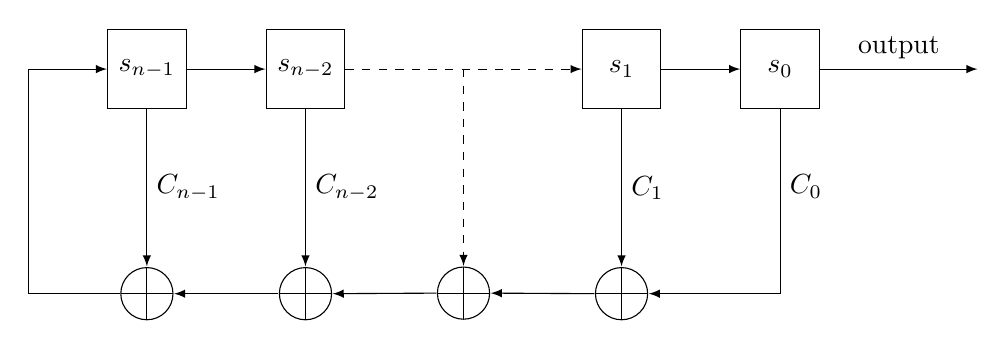
\begin{tikzpicture}


		\node[block                  ] (last_register) {$s_{n-1}$};
		\node[block, right = 1cm of last_register] (second_last_register) {$s_{n-2}$};
		\draw[line] (last_register.east) -- (second_last_register.west) ;

		\node[block, right = 3cm of second_last_register] (second_register) {$s_{1}$};
		\node[block, right = 1cm of second_register] (mid_register) {$s_{0}$};
		\draw[line] (second_register.east) -- (mid_register.west) ;

		\draw[dashed, line] (second_last_register.east) -- (second_register.west) ;

		\node[coordinate, right = 2cm of mid_register] (output_point) {};
		\draw[line] (mid_register.east) -- (output_point.west) node [midway, above] {output};

		\node[XOR, scale=2, below = 2cm of second_register] (first_xor) {};
		\draw[line] (second_register.south) -- (first_xor.north) node [midway, right] {$C_1$};
		\draw[line] (mid_register.south) |- (first_xor.east) node [pos=0.21, right] {$C_0$};

		\node[coordinate, right = 1.5cm of second_last_register] (h) {};
		\node[XOR, scale=2, below = 2.5cm of h] (mid_xor) {};
		\draw[line] (first_xor.west) -- (mid_xor.east) ;
		\draw[dashed, line] (h.south) -- (mid_xor.north) ;

		\node[XOR, scale=2, below = 2cm of second_last_register] (second_last_xor) {};
		\node[XOR, scale=2, below = 2cm of last_register] (last_xor) {};

		\draw[line] (second_last_register.south) -- (second_last_xor.north) node [midway, right] {$C_{n-2}$};
		\draw[line] (mid_xor.west) -- (second_last_xor.east) ;
		
		\draw[line] (second_last_xor.west) -- (last_xor.east) ;
		\draw[line] (last_register.south) -- (last_xor.north) node [midway, right] {$C_{n-1}$};

		\node[coordinate, left = 1cm of last_register] (return_point) {};
		
		\draw[line] (last_xor.west) -| (return_point) -- (last_register.west) ;




	\end{tikzpicture}
	\caption{Linear feedback shifter register of length $n$, with XOR gates.}
	\label{fig:lfsr}
\end{figure}


For PN sequences, there exists no formula for the cross-correlation of two different PN sequences. 
Exhaustive analysis is required to find out which sequences or entire sets have the cross-correlation characteristics that are good enough for the user's application.

The size of the code set is limited.
For a LFSR with $n$ registers, the maximum number of possible codes $C$ is given by \autoref{eq:num-of-pn-codes} \cite{mutagi1996pseudo}, where $P_i$ are the prime factors of $2^n - 1$ and $\alpha_i$ is the power of $i$th prime factor.

\begin{equation}
	\label{eq:num-of-pn-codes}
	C = \frac{1}{n} \prod \{ P_{i} ^ {(\alpha_i - 1)} \times (P_i - 1) \}
\end{equation}

For example when using a LFSR of size $n = 6$, $2^n - 1 = 63$, which can be factored into $3^2 \times 7$.
Giving $P_1 = 3$, $P_2 = 7$, $\alpha_1 = 2$ and $\alpha_2 = 1$.
Thus, the maximum number of codes is: $C = \frac{1}{6} \times \{ 3^{2 - 1} \times (3 - 1) \} \times \{ 7^{1 - 1} \times (7 - 1) \} = 6$.
Another example: Say there are going to be 144 user, so 144 codes are needed. 
This means a code length of 4095 chips.
















\subsection{Gold Sequences}

Gold sequences are a type of PN sequence. 
They are created by using two LFS registers as shown in \autoref{fig:gold-lfsr}.
In this figure there are two vectors $s$ and $t$ and two polynomials $C$ and $D$.
For a sequence to be constructed in this way that is a Gold sequence, only preferred pairs of polynomials can be used \cite{kedia2012comparative}.
When we have the polynomials $p(x)$ and $q(x)$, which are a preferred pair and produces the PN sequences $d_1$ and $d_2$ respectively, the resulting set of Gold codes is defined as can be seen in \autoref{eq:gold-def}, where $T^n$ represent the cyclic shift of $n$ bits.

\begin{equation}
	\label{eq:gold-def}
	Gold(d_1, d_2) = \{ d_1, d_2, d_1 \oplus d_2, d_1 \oplus Td_2, d_1 \oplus T^2d_2, \dotsc, d_1 \oplus T^{L - 1}d_2 \}
\end{equation}


\begin{figure}[h]
	\centering
	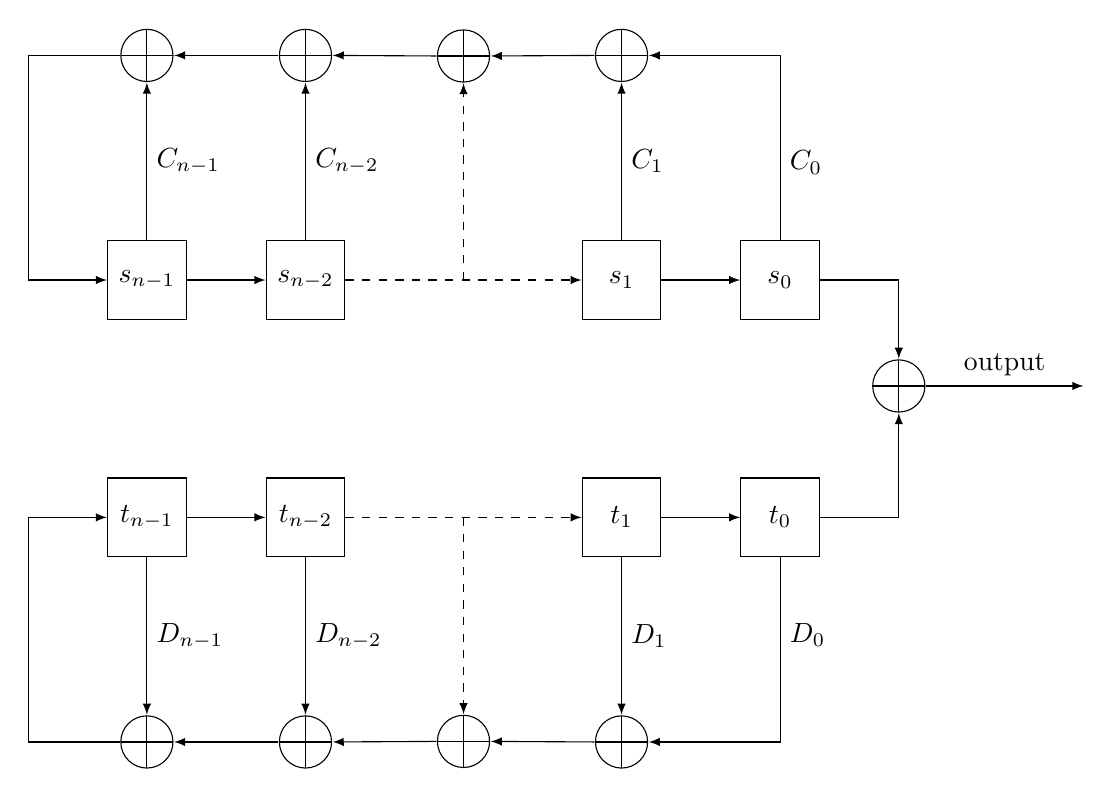
\begin{tikzpicture}

		\node[block                  ] (last_register1) {$s_{n-1}$};
		\node[block, right = 1cm of last_register1] (second_last_register1) {$s_{n-2}$};
		\draw[line] (last_register1.east) -- (second_last_register1.west) ;

		\node[block, right = 3cm of second_last_register1] (second_register1) {$s_{1}$};
		\node[block, right = 1cm of second_register1] (mid_register1) {$s_{0}$};
		\draw[line] (second_register1.east) -- (mid_register1.west) ;

		\draw[dashed, line] (second_last_register1.east) -- (second_register1.west) ;

		\node[coordinate, right = 1cm of mid_register1] (output_point1) {};

		\node[XOR, scale=2, above = 2cm of second_register1] (first_xor1) {};
		\draw[line] (second_register1.north) -- (first_xor1.south) node [midway, right] {$C_1$};
		\draw[line] (mid_register1.north) |- (first_xor1.east) node [pos=0.21, right] {$C_0$};

		\node[coordinate, right = 1.5cm of second_last_register1] (h1) {};
		\node[XOR, scale=2, above = 2.5cm of h1] (mid_xor1) {};
		\draw[line] (first_xor1.west) -- (mid_xor1.east) ;
		\draw[dashed, line] (h1.north) -- (mid_xor1.south) ;

		\node[XOR, scale=2, above = 2cm of second_last_register1] (second_last_xor1) {};
		\node[XOR, scale=2, above = 2cm of last_register1] (last_xor1) {};

		\draw[line] (second_last_register1.north) -- (second_last_xor1.south) node [midway, right] {$C_{n-2}$};
		\draw[line] (mid_xor1.west) -- (second_last_xor1.east) ;
		
		\draw[line] (second_last_xor1.west) -- (last_xor1.east) ;
		\draw[line] (last_register1.north) -- (last_xor1.south) node [midway, right] {$C_{n-1}$};

		\node[coordinate, left = 1cm of last_register1] (return_point1) {};
		
		\draw[line] (last_xor1.west) -| (return_point1) -- (last_register1.west) ;

		%%%%%%%%%%%%%%%%%%%%%%%%%%%%%%%%%%%%%%%%%%%%%%%%%%%%%%%%%%%%%%%%%%%%%%%%%%%%


		\node[block, below = 2cm of last_register1] (last_register) {$t_{n-1}$};
		\node[block, right = 1cm of last_register] (second_last_register) {$t_{n-2}$};
		\draw[line] (last_register.east) -- (second_last_register.west) ;

		\node[block, right = 3cm of second_last_register] (second_register) {$t_{1}$};
		\node[block, right = 1cm of second_register] (mid_register) {$t_{0}$};
		\draw[line] (second_register.east) -- (mid_register.west) ;

		\draw[dashed, line] (second_last_register.east) -- (second_register.west) ;

		\node[coordinate, right = 1cm of mid_register] (output_point) {};

		\node[XOR, scale=2, below = 2cm of second_register] (first_xor) {};
		\draw[line] (second_register.south) -- (first_xor.north) node [midway, right] {$D_1$};
		\draw[line] (mid_register.south) |- (first_xor.east) node [pos=0.21, right] {$D_0$};

		\node[coordinate, right = 1.5cm of second_last_register] (h) {};
		\node[XOR, scale=2, below = 2.5cm of h] (mid_xor) {};
		\draw[line] (first_xor.west) -- (mid_xor.east) ;
		\draw[dashed, line] (h.south) -- (mid_xor.north) ;

		\node[XOR, scale=2, below = 2cm of second_last_register] (second_last_xor) {};
		\node[XOR, scale=2, below = 2cm of last_register] (last_xor) {};

		\draw[line] (second_last_register.south) -- (second_last_xor.north) node [midway, right] {$D_{n-2}$};
		\draw[line] (mid_xor.west) -- (second_last_xor.east) ;
		
		\draw[line] (second_last_xor.west) -- (last_xor.east) ;
		\draw[line] (last_register.south) -- (last_xor.north) node [midway, right] {$D_{n-1}$};

		\node[coordinate, left = 1cm of last_register] (return_point) {};
		
		\draw[line] (last_xor.west) -| (return_point) -- (last_register.west) ;

		%%%%%%%%%%%%%%%%%%%%%%%%%%%%%%%%%%%%%%%%%%%%%%%%%%%%%%%%%%%%%%%%

		\node[XOR, scale=2, below = 1cm of output_point1] (gold_xor) {};
		\draw[line] (mid_register1) -| (gold_xor) ;
		\draw[line] (mid_register) -| (gold_xor) ;
		\node[coordinate, right = 2cm of gold_xor] (gold_output) {} ;
		\draw[line] (gold_xor.east) -- (gold_output.west) node [midway, above] {output};


	\end{tikzpicture}
	\caption{Two linear feedback shifter registers of length $n$, with XOR gates to produce a set of Gold sequences.}
	\label{fig:gold-lfsr}
\end{figure}

\begin{figure}
	\centering
	\includegraphics[width=\textwidth]{chapters/cdma-chapters/autocorr-gold.eps}
	\caption{Autocorrelation of one Gold sequence of length 1023.}
	\label{fig:autocorr-gold}
\end{figure}


\begin{figure}
	\centering
	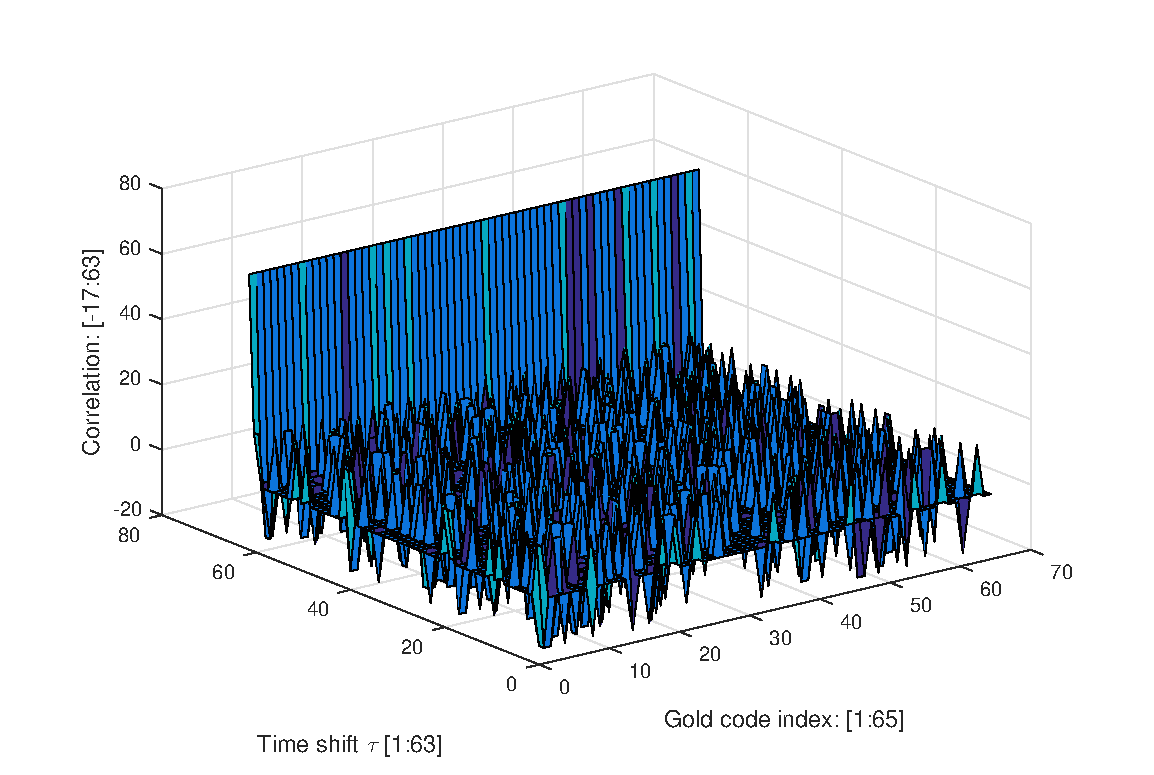
\includegraphics[width=\textwidth]{chapters/cdma-chapters/autocorr-gold-3d.eps}
	\caption{Autocorrelation of all Gold codes in the same set of length 63.}
	\label{fig:autocorr-gold-3d}
\end{figure}




The autocorrelation properties of Gold sequences are not as good as that of the PN sequences, as can be seen from \autoref{fig:autocorr-gold-3d}.
Apart from the original two PN sequences the autocorrelation values are not two-valued, but are four-valued.
See \autoref{eq:autocorr-gold} and \autoref{eq:gold-t(n)} for the autocorrelation properties of Gold sequences.

\begin{equation}
	\label{eq:autocorr-gold}
	R(\tau) = 
		\begin{cases}
			L    							& \quad \text{if } \tau = 0 \\
			\{ -t(n), \ -1, \ t(n) - 2  \} 	& \quad \text{if } \tau \neq 0 \\
		\end{cases}
\end{equation}

\begin{equation}
	\label{eq:gold-t(n)}
	t(n) = 
		\begin{cases}
			1 + 2^{\frac{n+1}{2}} & \quad \text{for odd } n \\
			1 + 2^{\frac{n+2}{2}} & \quad \text{for even } n \\
		\end{cases}
\end{equation}

See \autoref{eq:corsscorr-gold} and \autoref{eq:gold-t(n)} for the cross-correlation properties of Gold sequences \cite{mitra2008pseudo}.

\begin{equation}
	\label{eq:corsscorr-gold}
	R_{xy}(\tau) = 	\{ -t(n), -1, t(n) - 2  \} 
\end{equation}


From these equations it is clear to see that the absolute maximum cross-correlation is bounded by $t(n)$.

When $n$ is chosen to be odd, something can be said about the approximate frequency of occurrence of the cross-correlation values, see \autoref{tbl:freq-occurence-gold-cross-correlation} \cite{holmes2007spread}.

\begin{table}[h]
	\centering
	\begin{tabular}{ | l | l | }

		\hline
		$R_{xy}(\tau)$ 	& Frequency of occurrence	\\ \hline

		$-1$			& 0.5					 	\\ \hline
		$-t(n)$			& 0.25						\\ \hline
		$t(n) - 2$		& 0.25						\\ \hline

		

	\end{tabular}
	\caption{Table containing the approximate frequency of occurrence for all the cross-correlation values for $n$ odd.}
	\label{tbl:freq-occurence-gold-cross-correlation}
\end{table}

The Gold sequences posses good auto- and crosscorelation, suitable for a-synchronous usage.
\todo{Also state that this is extra good, because the LEDs/transmitters cannot be synchronized ???}
Also the codes scale well.
With a LFSR of $n$, the sequence length is $L = 2^n - 1$ and the number of sequences is $C = 2^n + 1$.

\todo{What information is really needed and which (like this table) is not necessary}












% !TeX root = ../../thesis.tex

\section{Mapping Problem}
\label{sec:mapping-problem}

The coding methods as discussed in \autoref{sec:orthogonal-sequences} and \autoref{sec:pn-sequences} are used in the field of telecommunication.
Since these signals are analog radio waves, the symbols are $+1$ and $-1$.
The orthogonal sequences generated via the Hadamard matrix can already be in this form, but the PN sequences contain only zeros and ones.
For the use with radio-signals the PN sequence is mapped to a form with $+1$ and $-1$, where the original $0$ is mapped to $+1$ and the original $1$ is mapped to $-1$.




The following proof \todo{Are we calling this a proof ??} shows how to calculate the correlation when the coding sequence consists of $+1$ and $-1$ symbols: 

\begin{proof}
	Let $s(t)$ be the received signal which is the composed signal of $m$ distinct codes.\\
	And let $c_i(t)$ be the code sequence $i$, and let $c_1(t)$ be the code for which we want to check if there is information there. \\

	\begin{align*}
		R(\tau)_{xy} = \displaystyle\sum_{t = 0} ^ {L - 1} x(t) \times y(t + \tau)	\tag{See \autoref{eq:correlation}}
		\\ \tau = 0,\ x = s(t),\ y = c_1(t)	
		\\ R(0)_{sc_{1}} = \displaystyle\sum_{t = 0} ^ {L - 1} s(t) \times c_1(t)
		\\ s(t) = \displaystyle\sum_{i = 1} ^ {m} c_i(t)														
		\\ R(0)_{sc_{1}} = \displaystyle\sum_{t = 0} ^ {L - 1}  \Bigg\{  c_1(t)	\times \displaystyle\sum_{i = 1} ^ {m} c_i(t) \Bigg\}
		\\ R(0)_{sc_{1}} = \displaystyle\sum_{t = 0} ^ {L - 1} \Bigg\{ c_1(t) \times c_1(t) + c_1(t) \times  \displaystyle\sum_{i = 2} ^ {m} c_i(t) \Bigg\} 
		\\ R(0)_{sc_{1}} = \displaystyle\sum_{t = 0} ^ {L - 1} c_1(t) \times c_1(t) + \displaystyle\sum_{t = 0} ^ {L - 1} \Bigg\{ c_1(t) \times  \displaystyle\sum_{i = 2} ^ {m} c_i(t) \Bigg\} 
		\\ R(0)_{sc_{1}} = L + \displaystyle\sum_{t = 0} ^ {L - 1} \Bigg\{ c_1(t) \times  \displaystyle\sum_{i = 2} ^ {m} c_i(t) \Bigg\} 
	\end{align*}

\end{proof}

So the result is $L$ plus the sum of all the other correlations. 
If the orthogonal sequences were used all the other correlations are zero.
If the Gold sequences were used each of the other correlations could be one of the values stated in \autoref{eq:corsscorr-gold}.
This is where the multiple access interference shows.



The above correlation calculation only holds up, when using a coding sequence which has the $+1$ and $-1$ symbols.
But when having LEDs which are modulating according to a sequence, the current draw is either on or off, a zero or a one.
This means a different correlation calculation is required.
First a formula for the mapping from $+1$ to zero and $-1$ to one is needed.
The formula can be found in \autoref{eq:radio-to-bin}, where $r$ denotes the $+1$ or $-1$ symbols and the outcome $b$ will be our binary value, i.e. $0$ or $1$.

\begin{equation}
	b = \frac{1 - r}{2}
	\label{eq:radio-to-bin}
\end{equation}


The previous proof can now be altered to incorporate the fact that the LEDs work with a one and zero state.


\begin{proof}
	Let $s(t)$ be the received signal which is the composed signal of $m$ distinct codes, which have symbols consisting of zero and one, which will be denoted be $c^b_i(t)$\\
	And let $c^r_i(t)$ be the code sequence $i$, and let $c^r_1(t)$ be the code for which we want to check if there is information there. \\
	Where $c^r_i(t)$ denotes a code sequence consisting of symbols $-1$ and $+1$.

	\begin{align*}
	T(\tau)_{xy} = \displaystyle\sum_{t = 0} ^ {L - 1} x(t) \times y(t + \tau)	\tag{See \autoref{eq:correlation}}
	\\ \tau = 0,\ x = s(t),\ y = c^r_1(t)
	\\ T(0)_{sc^r_{1}} = \displaystyle\sum_{t = 0} ^ {L - 1} s(t) \times c^r_1(t)	
	\\ s(t) = \displaystyle\sum_{i = 1} ^ {m} c^b_i(t)
	\\ T(0)_{sc^r_{1}} = \displaystyle\sum_{t = 0} ^ {L - 1} \Bigg\{  c^r_1(t)	\times \displaystyle\sum_{i = 1} ^ {m} c^b_i(t) 	\Bigg\}
	\\ T(0)_{sc^r_{1}} = \displaystyle\sum_{t = 0} ^ {L - 1} \Bigg\{  c^r_1(t)	\times \displaystyle\sum_{i = 1} ^ {m} \frac{1 - c^r_i(t)}{2}  	\Bigg\}
	\\ T(0)_{sc^r_{1}} = \frac{m}{2} \times \displaystyle\sum_{t = 0} ^ {L - 1} c^r_1(t) - \frac{1}{2} \times \displaystyle\sum_{t = 0} ^ {L - 1}  \Bigg\{ c^r_1(t) \times \displaystyle\sum_{i = 1} ^ {m} c^r_i(t) \Bigg\}
	\end{align*}

\end{proof}

This correlation calculation, denoted by $T$ now shows a different result than the previous result $R$.
Where $R = \displaystyle\sum_{t = 0} ^ {L - 1}  \Bigg\{  c_1(t)	\times \displaystyle\sum_{i = 1} ^ {m} c_i(t) \Bigg\}$ and $T = \frac{m}{2} \times \displaystyle\sum_{t = 0} ^ {L - 1} c^r_1(t) - \frac{1}{2} \times \displaystyle\sum_{t = 0} ^ {L - 1}  \Bigg\{ c^r_1(t) \times \displaystyle\sum_{i = 1} ^ {m} c^r_i(t) \Bigg\}$.
We can write it such that $R$ will become a function of $T$: 

\begin{proof}

	\begin{align*}
	T = \frac{m}{2} \times \displaystyle\sum_{t = 0} ^ {L - 1} c^r_1(t) - \frac{1}{2} \times R
	\\ R = m \times \displaystyle\sum_{t = 0} ^ {L - 1} c^r_1(t) - 2 \times T
	\end{align*}

\end{proof}

The sum of the sequence depends on the sequence used, when using orthogonal codes the sum will be zero, see \autoref{sec:orthogonal-sequences}.
If the sum is equal to zero, the factor $m$ will not matter.
However when the sequence used is a PN sequence or a balanced Gold sequence, the sum will be $-1$, This means: $R = -m - 2 \times T$, and then $m$, the number of signals, is important.
When using an unbalanced Gold sequence, the sum if that sequence can be calculated on the spot.











% !TeX root = ../../thesis.tex

\chapter{Hardware Design}
\label{chp:hardware-design}




The codes that will be assigned to each LED have now been introduced.
Now, hardware is needed to put the theory of those codes into practice.
Since hardware will never behave exactly like the software simulations, this chapter will discuss the existing hardware that is out there.
Then, the shortcomings of the hardware are highlighted and custom hardware is introduced.
First the DC case is considered and then the AC case.



% !TeX root = ../../../thesis.tex

\section{DC Environment}
\label{sec:dc-environment}





In a DC environment, the code framework works well because the DC power signal is an easy signal to understand and work with.
For example, in \autoref{fig:dc-voltage-and-current-example} the voltage output of a DC power supply can be seen.
A load is switched on and off, and the current that flows over time can also be seen in the figure.
This switching causes the current to be a square wave with sharp edges.
The current is zero when the load is off and the current is a constant value for when the load is on.
This is the signal for one load.
If multiple of these current signatures will be aggregated, it will still be a square wave without distortions.

\begin{figure}[ht]
  \centering
  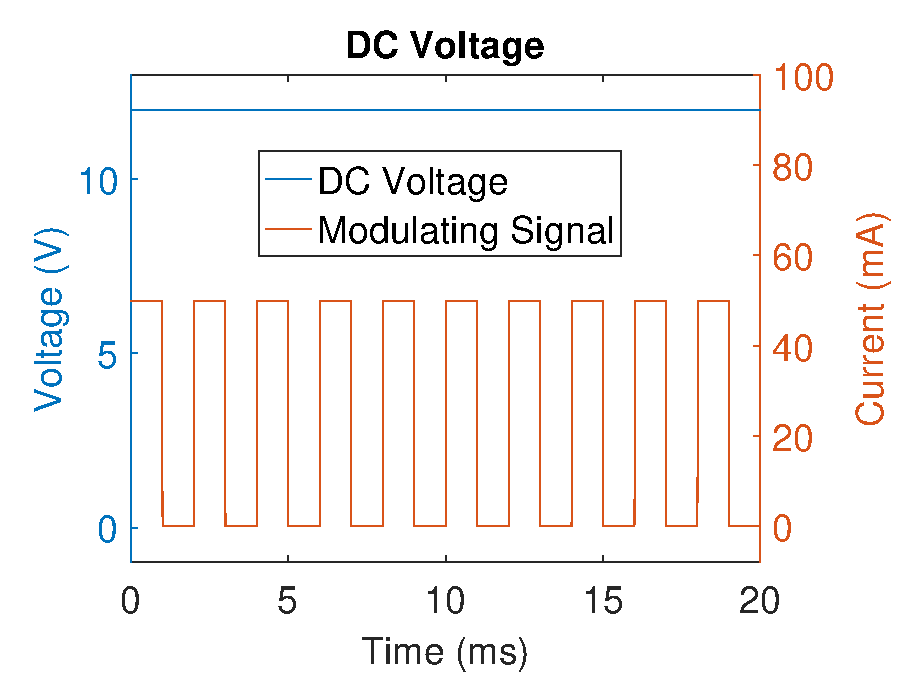
\includegraphics[angle=0,width=0.5\textwidth]{chapters/hardware-chapters/DC/dc-voltage-and-current-example.eps}
  \caption{Voltage of a DC power supply, along with the current of a switching load.}
  \label{fig:dc-voltage-and-current-example}
\end{figure}



This is the ideal way the modulator for an LED must work.
In the next sections, the hardware for the modulator will be explained as well as how the current will be measured to extract the encoded information and finally a testbed will be presented. 





% !TeX root = ../../../../thesis.tex

\subsection{Modulator}

	The task of the modulator is to switch the LED on or off based on the ID that is assigned to the light fixture.
	It is the responsibility of this piece of hardware to translate the ID into the unique current signature.


	The way an LED (Light Emitting Diode) works, is that current has to flow through it in order for it to emit light.
	In other words, an LED is controlled via current, it is not controlled by applying a voltage to it.
	When a certain amount of current flows through the LED, a certain amount of voltage will drop over the LED.

	The easiest way to make an LED emit light, is to put a current limiting resistor in series with a voltage source and an LED.
	A schematic can be seen in \autoref{fig:dc-led-resistor}.
	But there exists no ideal DC power supply.
	Depending on the load, the provided voltage of the power supply may fluctuate.
	Due to the fluctuation of the provided voltage, the LED can start to change in brightness.
	The current that flows through the LED is a function of the voltage over the resistor and the value of the resistor: $I = \frac{U}{R}$.
	So if $U$, the provided voltage, is fluctuating, the current that flows through the LED, $I$, will also fluctuate.
	This causes the brightness of the LED to fluctuate.


	A better way to power an LED, is by using a current source.
	Where an ideal voltage source will always deliver a certain amount of voltage independent of the load, a current source will always deliver a certain amount of current independent of the load.
	If a constant amount of current flows through the LED, the brightness will not fluctuate.
	In \autoref{fig:dc-led-current-source} a schematic can be seen, which shows an example of a current source powering an LED.
	This current source can be toggled on and off via a 0 V or 3.3/5 V signal, coming from a micro-controller, uC in the schematic.


	\begin{figure}[t]
		\centering
		\begin{minipage}[b]{0.3\textwidth}
			\includegraphics[width=\textwidth]{chapters/hardware-chapters/DC/dc-modulator/dc-led-resistor.jpg}
			\caption{Simplest way to power an LED.}
			\label{fig:dc-led-resistor}
		\end{minipage}
		\hfill
		\begin{minipage}[b]{0.5\textwidth}
			\includegraphics[width=\textwidth]{chapters/hardware-chapters/DC/dc-modulator/dc-led-current-source.jpg}
			\caption{Current source powering an LED.}
			\label{fig:dc-led-current-source}
		\end{minipage}
	\end{figure}

	By using a current source, two benefits can be identified:

	\begin{itemize}
		
		\item Since the current that flows through the LED is constant, the LED will not flicker.

		\item The current source will make sure that the current that is drawn, is either zero or some constant value depending on the bit that is being encoded.
		This will yield a signal with two distinct values.
		When multiple of these signals are aggregated and measured by a smart-meter, the measured signal will also have distinct values.
		This signal will make it easy to decode the information that was encoded by the modulators.

	\end{itemize}

% !TeX root = ../../../../thesis.tex

 \subsection{Current Sampler}

	Now that the hardware is created to translate the IDs of the LEDs into a unique current signature, we also need a way to measure the current.
	The measured current can then be processed by a micro-controller.
	And in turn it can be identified which LEDs are on and which are off.

	In the interest of time the most simple manner was chosen to measure the current for the DC hardware.
	Other options are available for measuring current and they will be discussed in the AC part.
	The most simple way to measure current is by using a series resistor.
	The resistance does not variate and therefor no noise is introduced in the sampled signal.
	The resistor is placed in series between the DC power supply and the LEDs.
	The voltage drop over the resistor is linearly proportional to the current that flows through the resistor, according to Ohm's Law $U = R \times I$.
	If the value of the resistor is chosen such that the maximum voltage will never exceed the rated voltage for a micro-controller, it can be directly measured by the micro-controller's ADC in question.

% !TeX root = ../../../../thesis.tex

\subsection{Testbed}
	\label{subsec:dc-testbed}

	To be able to test all aspects of the system a testbed was created.
	This testbed will allow the testing of the correlation calculations as discussed in \autoref{sec:mapping-problem}, the interference solutions (\autoref{subsec:continuous-method-modulation}), and the performance of the modulator and current-sampler.


	\begin{figure}[ht]
		\centering
		\includegraphics[angle=0,width=0.6\textwidth,height=.9\textheight,keepaspectratio]{chapters/hardware-chapters/DC/dc-test-bed/dc-test-bed-picture.JPG}
		\caption{Picture of the DC testbed, showing the six LED strips, current sources, current sampler and an Arduino board.}
		\label{fig:dc-test-bed-picture}
	\end{figure}

	\begin{figure}[ht]
		\centering
		\includegraphics[angle=0,width=1.0\textwidth,keepaspectratio]{chapters/hardware-chapters/DC/dc-test-bed/dc-test-bed-architectural.JPG}
		\caption{Architectural overview of the DC testbed. Six LED modulators are connected in parallel with each other and in series with the current sampler.}
		\label{fig:dc-test-bed-architectural}
	\end{figure}


	The testbed works with a DC power supply and has six individual controllable current sources.
	Each current source powers one LED fixture.
	The testbed itself can be seen in \autoref{fig:dc-test-bed-picture} and an architectural overview of how everything is connected to each other can be seen in \autoref{fig:dc-test-bed-architectural}.


	The aim of the testbed was to use commercial LEDs. 
	The LED fixtures used in this testbed all came from the same commercial LED, which can be found in \cite{commercial-230v-ac-led-aliexpress}.
	A picture of the LED can be seen in \autoref{fig:ac-commercial-230v-ac-led}.
	The strips are taken out of this commercial LED and used individually for this testbed.


	The current is measured by a series resistor and fed to the ADC of a micro-controller.
	The entire schematic of the DC testbed can be found in \autoref{app:dc-test-bed}. 

	The current sources and therefore the LEDs, can be toggled on and off by a micro-controller.
	By toggling the current sources on and off, the current that flows through the series resistor will change accordingly.
	A change of voltage over the series resistor can then be measured by the ADC.

	The measured current from the DC testbed can be seen in \autoref{fig:raw-dc-test-bed-data-short}.
	In this experiment, all six LEDs are modulating with the unique ID that was assigned to each LED.
	The voltage drop over the resistor is measured with the ADC.
	The raw ADC value can be seen on the left y-axis and the calculated aggregated current that is drawn can be seen on the right y-axis.
	From this figure seven distinguishable states can be seen.
	When there are no LEDs on, all LEDs are encoding a `0' data bit, the current is zero.
	When one of the six LEDs is transmitting a `1' data bit, the current jumps to roughly 50 mA.
	When two of the six LEDs are encoding a `1', the current is roughly 100 mA and so on.


	\begin{figure}
		\centering
		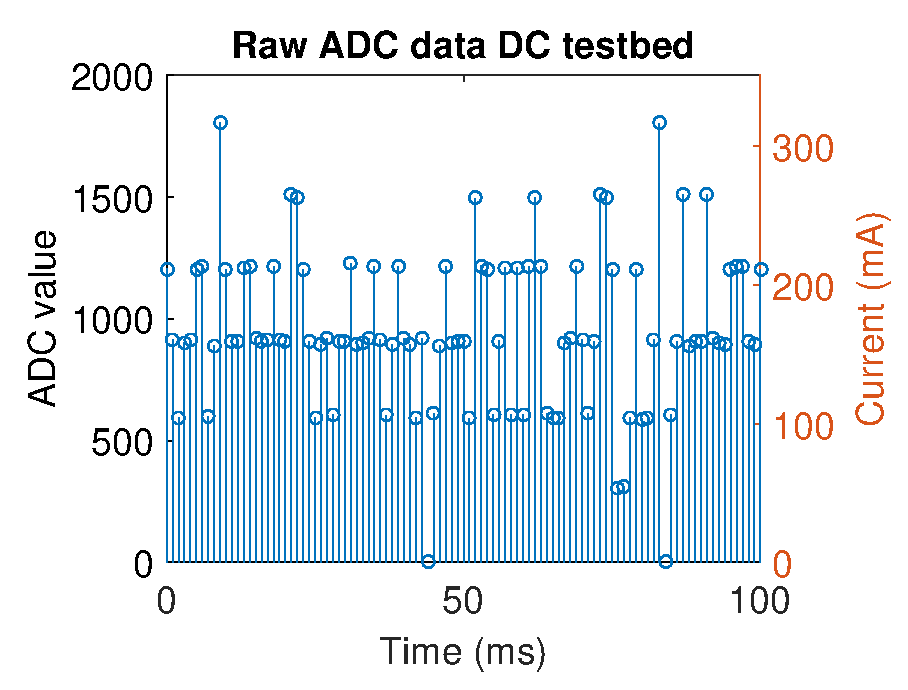
\includegraphics[angle=0,width=0.7\textwidth,keepaspectratio]{chapters/hardware-chapters/DC/dc-test-bed/dc-test-bed-raw-data.eps}
		\caption{Raw current data from the DC testbed with the six LEDs modulating with their unique IDs.}
		\label{fig:raw-dc-test-bed-data-short}
	\end{figure}



	An evaluation of this testbed is done in \autoref{subsec:dc-testbed-eval} where a longer signal will be shown along with correlation data to identify if a certain LED is on, while the other LEDs are modulating and thereby causing interference.













% !TeX root = ../../../thesis.tex

\section{AC Environment}
\label{sec:ac-environment}




The translation from an ID, that is assigned to a light fixture, to a unique current signature is more difficult in an AC environment compared to the DC environment.
This is due to the supplied voltage.
In a DC environment, the voltage is a constant value, but in an AC environment the supplied voltage is a sinusoidal wave.
This means that the voltage will be both positive and negative.
In the Netherlands the AC has an RMS voltage of 230 V and a frequency of 50 Hz.

In the next subsections, we will first describe existing hardware and their limitations.
Then new hardware is proposed to solve the limitations of the existing hardware.
Finally, the AC testbed is showcased.




% !TeX root = ../../../../thesis.tex


\subsection{Modulator}	
\label{subsec:ac-modulator}

The job of the modulator in an AC environment, is the same as in a DC environment.
Just like in the DC environment, when a `0' has to be encoded the current should be zero and when a `1' has to be encoded the current should be some constant value.
The transition between a `0' and `1' should be fast, so that a square wave is created, just like in the DC case.

If the translation is done in this manner, the mapping between the code sequence symbols and the current is clear and the aggregated current drawn by multiple lights will also be a square wave, which will allow for decoding the information.
Next, existing hardware is investigated if these solutions will translate the IDs into a current draw which is similar to what has just been discussed above. 



\input{chapters/hardware-chapters/AC/ac-modulator/smps-led/smps-led}




	\begin{figure}
		\centering
		\begin{minipage}[b]{0.45\textwidth}
			\includegraphics[width=\textwidth]{chapters/hardware-chapters/AC/ac-modulator/smps-led/smps-led-and-smps-picture.jpg}
			\caption{Picture of a commercial LED light fixture with a DC SMPS.}
			\label{fig:ac-smps-led-and-smps-picture}
		\end{minipage}
		\hfill
		\begin{minipage}[b]{0.45\textwidth}
			\centering
			\includegraphics[angle=0,width=0.5\textwidth]{chapters/hardware-chapters/AC/ac-modulator/commercial-230v-ac-led/commercial-ac-led-picture.jpg}
			\caption{Picture of a commercial 230 V AC LED light fixture.}
			\label{fig:ac-commercial-230v-ac-led}
		\end{minipage}
	\end{figure}




\input{chapters/hardware-chapters/AC/ac-modulator/commercial-230v-ac-led/commercial-230v-ac-led}


\input{chapters/hardware-chapters/AC/ac-modulator/custom-hardware/ac-custom-hardware}















% !TeX root = ../../../../thesis.tex


\subsection{Current Sampler}
\label{subsec:ac-current-sampler}


Now that there exists a solution to encode the ID of an LED into the current draw, as explained in \autoref{subsec:ac-modulator}, it is now time to explore the possibilities to measure the current.
The measured current can then be processed by a micro-controller, and then the status of the LEDs can be determined.


To measure the AC current, first existing solutions were investigated.
One such a product is a `Hall Effect-Based Linear Current Sensor' \cite{hall-ac-current-sensor-datasheet}.
Based on the Hall effect, this sensor outputs a voltage which is proportional to the current that goes through the sensor.
This sensor has the issue that the noise is larger than the voltage signal which is outputted using the provided LEDs.
According to \cite{hall-ac-current-sensor-datasheet}, the highest sensitivity is $185$ mV / A and the noise is rated at $21$ mV.
The commercial LED fixtures which were provided, are rated at $15$ Watts.
With the 230 V AC, this works out to a current of $I = \frac{P}{U} = \frac{15}{230} = 0.065$ A.
At that current the output voltage will be $185 \times 0.065 = 12$ mV.
The noise of the output is $21$ mV, which is almost double the output voltage when one LED is on.
This sensor would not be able to reliably detect one or two LEDs.



Another solution has to be used to overcome the noise problem of the Hall effect sensor.
This solution has two parts: The current sampler itself and a triggering circuit.

The triggering circuit is needed to know when the modulators start and stop encoding the ID.
This will help the smart-meter, by telling it when to start and stop looking for the IDs of the LEDs.
The triggering circuit is the same circuit that was used for the modulator, which was explained in \autoref{subsec:ac-modulator}.
The part which samples the current will be explained next, but first an overview is given of how the different parts of the smart-meter are connected in \autoref{fig:ac-current-sampler-architectural}.
The meter is placed in series with an incoming AC power-line and the LEDs will be connected with the AC output.
The current-sampler forwards information about the current draw to a micro-controller for processing.
And the triggering circuit detects when the voltage is high enough for modulation for the LEDs. 


\begin{figure}[h]
	\centering
	\includegraphics[angle=0,width=0.7\textwidth,keepaspectratio]{chapters/hardware-chapters/AC/ac-current-sampler/ac-current-sampler-architectural.JPG}
	\caption{Architectural overview of the AC current sampler.}
	\label{fig:ac-current-sampler-architectural}
\end{figure}


For the current-sampler itself a resistor will be used, since this approach ensures that no noise will be introduced to the sampled current signal.
As could be seen from \autoref{fig:custom-modulator-current-source}, the current that flows is both positive and negative, due to the nature of the AC that is used.
This means that the voltage that is measured over the resistor will also be positive and negative.
An ADC (Analog-to-Digital Converter) cannot measure a negative voltage.
So the voltage over the resistor is summed with another voltage to ensure that the ADC will always measure a positive voltage.
This other voltage comes from a reference voltage IC \cite{lm336z-ref-voltage-datasheet}, which outputs a very stable reference voltage often used in scenarios where an ADC is used to measure analog signals.

At this point the ADC is measuring the voltage over a resistor which is in series with the ground (N) or phase (L) of the 230 V AC.
For safety reason the ADC must now be electrically isolated from the micro-controller, such that no harm can come from even touching the micro-controller.
To this end, an SPI isolating chip was used \cite{iso7241m-spi-isolator-datasheet} to electrically isolate the SPI signals between the ADC and the micro-controller.




This solution to sample current with an external ADC can sample the current with an high frequency ($> 10$ kHz) with no noise introduced in the signal.
The full schematic of the current sampler can be found in \autoref{app:custom-current-sampler-schematic}.





% !TeX root = ../../../../thesis.tex


\subsection{Testbed}
\label{subsec:ac-testbed}

\begin{figure}[h]
	\centering
	\includegraphics[angle=0,width=\textwidth,height=.9\textheight,keepaspectratio]{chapters/hardware-chapters/AC/ac-test-bed/ac-test-bed-picture}
	\caption{Picture of the AC testbed, consisting of three modulators each connected to three commercial LEDs. The modulators are controlled via three separate Arduino boards. Finally there is the current sampler with its own Arduino board.}
	\label{fig:ac-test-bed-picture}
\end{figure}



An overview of the AC testbed can be found in \autoref{fig:ac-test-bed-architectural-overview} and a picture of the actual testbed itself can be seen in \autoref{fig:ac-test-bed-picture}.
In the testbed three commercial LEDs are used which are powered by the custom modulators as explained in \autoref{subsec:ac-modulator}.
Arduino boards are controlling the modulators.
The modulators are connected in parallel. 
And in series is the custom current-sampler to measure the current and decode the information that the modulators encode into the current draw.
The custom current-sampler has its own Arduino board to process the current signal.
All Arduino board are stand-alone, and are not connected to each other in any way.


\begin{figure}[h]
	\centering
	\includegraphics[angle=0,width=0.9\textwidth,keepaspectratio]{chapters/hardware-chapters/AC/ac-test-bed/ac-test-bed-architectural.JPG}
	\caption{Architectural overview of the AC testbed. Three LED modulators, with switches to turn the LED on and off, are connected in parallel with each other and in series with the current sampler.}
	\label{fig:ac-test-bed-architectural-overview}
\end{figure}



In \autoref{fig:raw-ac-testbed-adc-data-testbed} the raw data that is collected by the smart-meter can be seen.
The current signal is shown here alongside the trigger output.
In the raw data the charging peaks of the capacitor of the non-disturbing voltage source can be seen.
Note that these peaks indeed do not interfere with the modulated data.
The modulated data and the charging peaks can be filtered out by the micro-controller with the help of the triggering circuits logical output.
As discussed in \autoref{subsec:ac-modulator}, the time that is available for modulation is 8 ms in a 10 ms period.
Depending on the length of the ID $L$ and the modulation frequency $f$, it can happen that this window of 8 ms is too small to encode the entire ID.
In this case, the remaining bits of the ID which could not fit inside the first 8 ms window, will be transmitted in the next window.
An evaluation with this testbed will be done in \autoref{subsec:ac-evaluation}.



\begin{figure}[h]
  \centering
  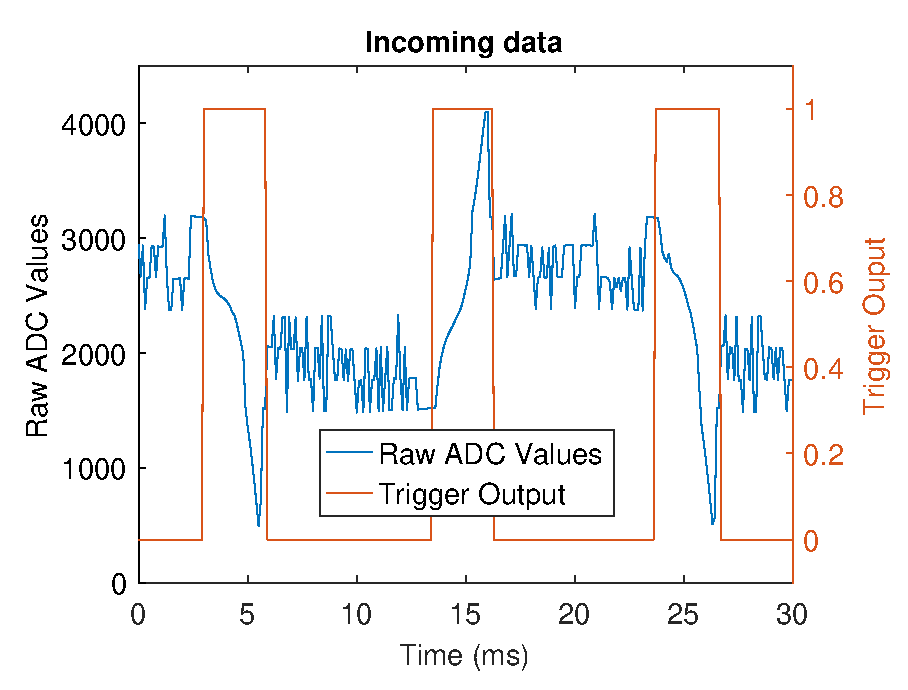
\includegraphics[width=0.7\textwidth]{chapters/evaluation-chapters/hardware/ac/raw-ac-testbed-adc-data.eps}
    \caption{Incoming data to the AC current sampler. The raw ADC values are plotted as well as the triggering circuit output.}
  \label{fig:raw-ac-testbed-adc-data-testbed}
\end{figure}



% !TeX root = ../../thesis.tex

\chapter{Evaluation}
\label{chp:evaluation}


In this chapter the designed hardware and software will be evaluated, for both the DC and the AC testbeds.
After that, simulation will evaluate the scalability of the setups.

When there is a system for which we can classify the results as false/true-positives and false/true-negatives, we can evaluate the system's performance by investigating the precision and recall.
The definitions of precision and recall can be found in \autoref{eq:precision} and \autoref{eq:recall} respectively, where $tp$ stands for the number of true-positives, $fp$ stand for the number of false-positives and $fn$ stand for the number of false-negatives.

\begin{equation}
	\label{eq:precision}
	\text{Precision } = \frac{tp}{tp + fp}
\end{equation}

\begin{equation}
	\label{eq:recall}
	\text{Recall } = \frac{tp}{tp + fn}
\end{equation}

This method provides two metrics to consider.
Ideally we want only one metric to consider and draw conclusion based on that.
We can take the weighted average of the two metrics.
This is called the F-measure \cite{sokolova2009systematic} and is the harmonic mean of the precision and recall.
The definition of the F-measure can be seen in \autoref{eq:F-measure}.

\begin{equation}
	\label{eq:F-measure}
	F = 2 \times \frac{\text{precision} \times \text{recall}}{\text{precision} + \text{recall}}
\end{equation}






% !TeX root = ../../../thesis.tex

\section{Hardware}
\label{sec:hardware-evaluation}

The following two section will describe the evaluation of the designed hardware and software.
All attached LEDs will be modulating with a different Gold code per LED, from the same set.
The raw ADC signal will be showed as well as the steps to process that signal to be able to do correlation calculations with, if necessary.
Next, the correlation graph will be showed for a Gold code that is present in the received signal as well as the correlation graph for a Gold code from the same set which is not present in the received signal.
Finally the F-measure will be showed for these correlation graphs.


% !TeX root = ../../../../thesis.tex

\subsection{DC}
\label{subsec:dc-testbed-eval}

The DC testbed has six LEDs, as explained in \autoref{subsec:dc-testbed}.
Therefor six Gold codes will be used for the LEDs with a seventh code used to represent an LED in an off state.
From \autoref{tbl:correlation-gold-families}, we can see that for $m = 6$, where $m$ is the number of simultaneous transmitters such that no destructive interference takes place, requires a code length of 511 or higher.
With the DC testbed the experiments have been performed with a constant modulation frequency of 1 kHz.
Every two successive samples are $\frac{1}{1000} = 1$ ms apart.

In \autoref{fig:raw-dc-testbed-adc-data-n=9} the raw ADC from the DC testbed can be seen.
The left y-axis represents the raw ADC data and the right y-axis is converted to current.
Six LEDs are simultaneous continuously modulating with different starting times.
From the figure, seven horizontal lines can be seen.
Each line represents how many LEDs are on, none through six.
This raw data is already in a form for which we can start calculating the correlation with a Gold sequence, no additional signal processing is needed.

In \autoref{fig:correlation-dc-testbed-n=9}, the correlation for one Gold sequence can be seen, which is also one of the sequences used to modulate an LED and the correlation for the extra Gold sequence can be seen, which is not part of the sequences used to modulate any LED and represent the LED is an off state.
All the correlation results from the Gold code used to modulate and LED with, stay below the threshold (See \autoref{eq:T}) except for the noticeable peaks.
These peaks indicate that the LED is on, which in fact is the case.
These peaks occur when the correlation is calculated when there is no time shift as already shown in \autoref{fig:autocorr-gold}.
The correlation results from the extra code all stay below the threshold, meaning the LED represented by this code is off, which is that case.

Since all the correlation levels are below the threshold, and the peaks are above the threshold, every result is correct.
There are only true positives and true negatives.
So the precision, recall and the F-measure are all equal to $1$ according to \autoref{eq:precision}, \autoref{eq:recall} and \autoref{eq:F-measure}, respectively.

\begin{figure}[!tbp]
  \centering
  \begin{minipage}[b]{0.49\textwidth}
    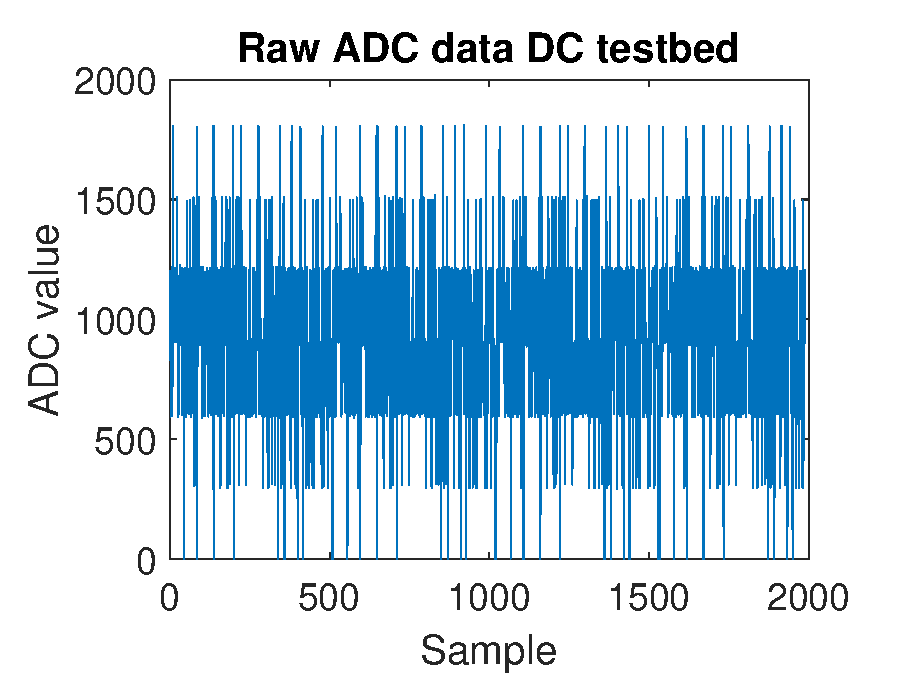
\includegraphics[width=\textwidth]{chapters/evaluation-chapters/hardware/dc/raw-dc-testbed-adc-data-n=9.eps}
    \caption{Raw ADC data from the DC testbed. With seven distinguishable entries, following the on-state of the combinations of LEDs. With a sequence length of 511.}
	\label{fig:raw-dc-testbed-adc-data-n=9}
  \end{minipage}
  \hfill
  \begin{minipage}[b]{0.49\textwidth}
    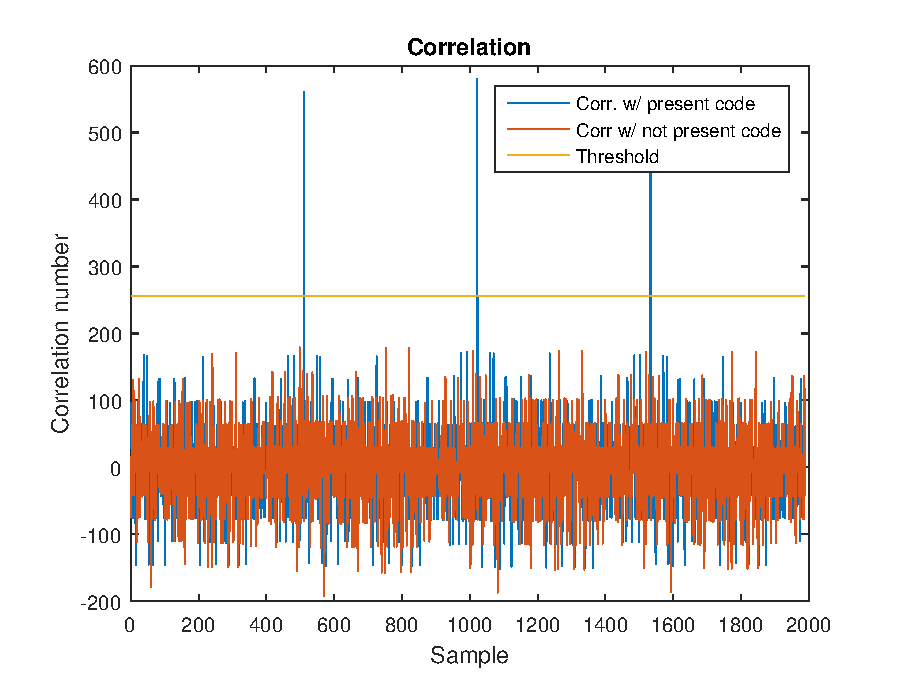
\includegraphics[width=\textwidth]{chapters/evaluation-chapters/hardware/dc/correlation-dc-testbed-n=9.eps}
    \caption{Correlations results from Gold sequences which are and which are not present, with the decision threshold. With a sequence length of 511.}
	\label{fig:correlation-dc-testbed-n=9}
  \end{minipage}
\end{figure}

To show how the F-measure would behave when there are false positives and/or false negatives a different Gold set is chosen.
A length of 127 is chosen, since it may only have three simultaneous continuously modulating LEDs (\autoref{tbl:correlation-gold-families}).
Again the six LEDs are simultaneous continuously modulating with different starting times.
For which the raw ADC can be seen in \autoref{fig:raw-dc-testbed-adc-data-n=7} on the left y-axis and on the right y-axis the current.
And the correlation can be found in \autoref{fig:correlation-dc-testbed-n=7}.
In the correlation figure, peaks can be seen that cross the threshold line, which are the autocorrelation peaks of the sequence.
They are supposed to be there.
But also other results can be seen to cross the threshold line.
These are the false positives, they occur because this code length can not support this much simultaneous transmitters.
The F-measure in time for these correlation results can be found in \autoref{fig:f-measure-dc-testbed-n=7}.
And the precision, recall and F-measure can be found in \autoref{fig:eval-metrics-dc-testbed-n=7}.


\begin{figure}[!tbp]
  \centering
  \begin{minipage}[b]{0.49\textwidth}
    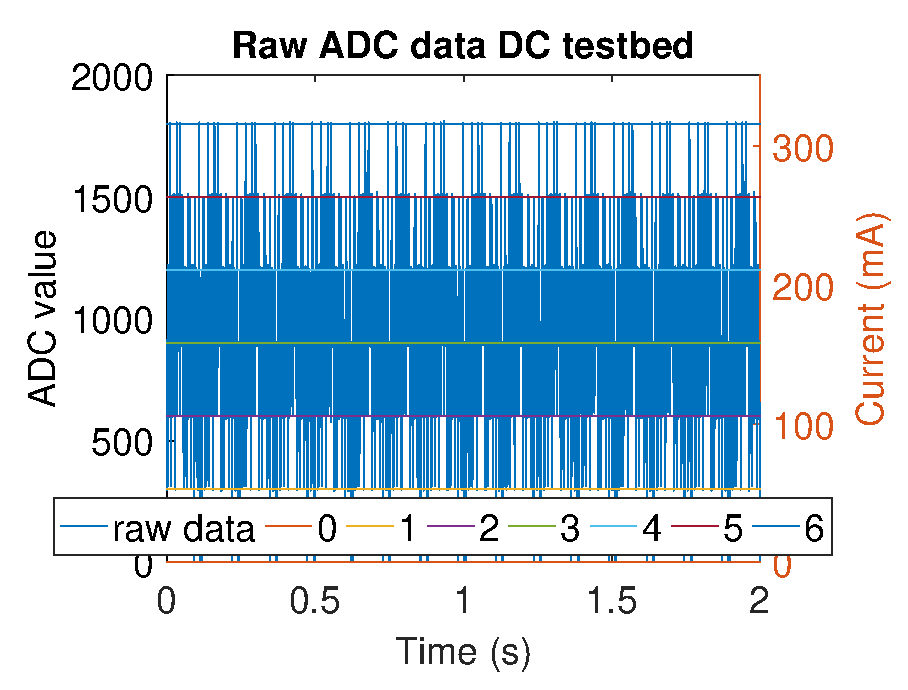
\includegraphics[width=\textwidth]{chapters/evaluation-chapters/hardware/dc/raw-dc-testbed-adc-data-n=7.eps}
    \caption{Raw ADC data from the DC testbed. With seven distinguishable entries, following the on-state of the combinations of LEDs. With a sequence length of 127  on the DC testbed.}
	\label{fig:raw-dc-testbed-adc-data-n=7}
  \end{minipage}
  \hfill
  \begin{minipage}[b]{0.49\textwidth}
    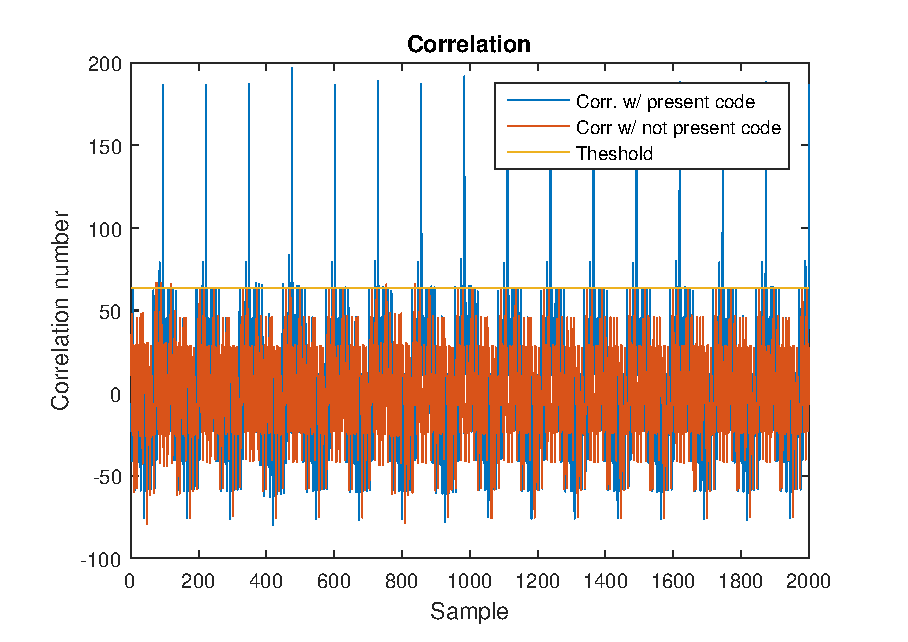
\includegraphics[width=\textwidth]{chapters/evaluation-chapters/hardware/dc/correlation-dc-testbed-n=7.eps}
    \caption{Correlations results from Gold sequences which are and which are not present, with the decision threshold. With a sequence length of 127 on the DC testbed.}
	\label{fig:correlation-dc-testbed-n=7}
  \end{minipage}
\end{figure}


\begin{figure}[!tbp]
  \centering
  \begin{minipage}[b]{0.49\textwidth}
  	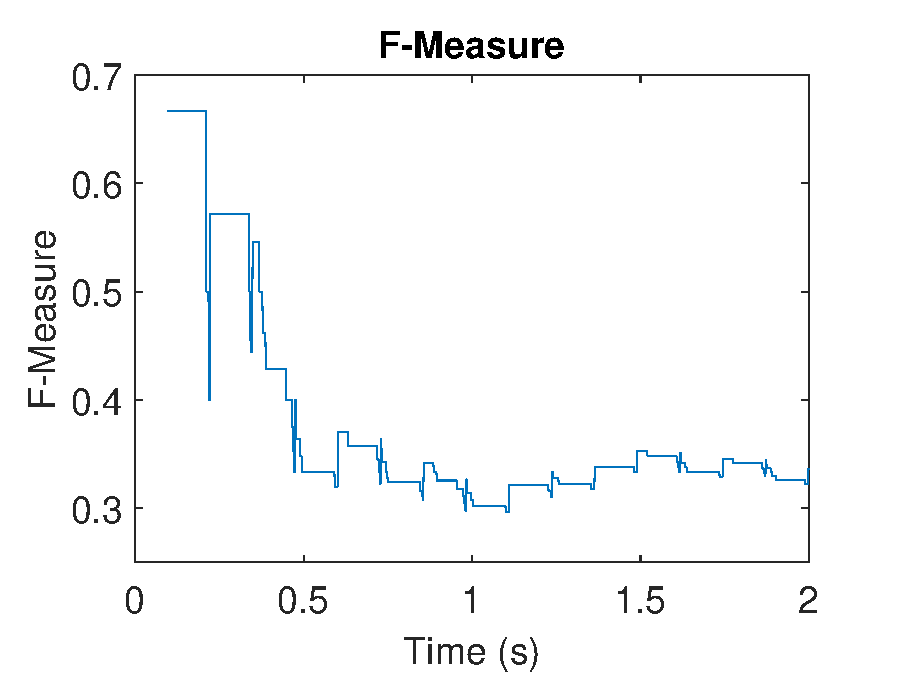
\includegraphics[width=\textwidth]{chapters/evaluation-chapters/hardware/dc/f-measure-dc-testbed-n=7.eps}
  	\caption{F-Measure of DC testbed correlation (\autoref{fig:correlation-dc-testbed-n=7}), with sequence length of 127.}
  	\label{fig:f-measure-dc-testbed-n=7}
  \end{minipage}
  \hfill
  \begin{minipage}[b]{0.49\textwidth}
    \includegraphics[width=\textwidth]{chapters/evaluation-chapters/hardware/dc/eval-metrics-dc-testbed-n=7.eps}
    \caption{Evaluation metrics of DC testbed correlation (\autoref{fig:correlation-dc-testbed-n=7}), with sequence length of 127.}
    \label{fig:eval-metrics-dc-testbed-n=7}
  \end{minipage}
\end{figure}




% !TeX root = ../../../../thesis.tex

\subsection{AC}


% !TeX root = ../../../thesis.tex

\section{Simulation}
\label{sec:simulation-evaluation}

In \autoref{sec:hardware-evaluation} the evaluation of the hardware and software was shown using the continuous transmission method, as detailed in \autoref{subsec:continuous-method-modulation}.
Since this is already been evaluated and proven, in this simulation section the scalability of a larger system will be evaluated, using the probabilistic method as explained in \autoref{subsec:probabilistic-method-modulation}.


Before the actual simulation itself, parameters such as $\epsilon$ need to be set.
1 - $\epsilon$, is the probability that for every point in time the number of LEDs that are modulating will not exceed $m$, as discussed in \autoref{subsec:probabilistic-method-modulation}.
This will determine if interference can occur and therefor the overall accuracy and correctness of the system.

For the rest of this simulation a Gold sequence set with length 127 will be used for the assessment.
This set has 129 unique Gold sequences.

This simulation does the following: 

\begin{itemize}

	\item For the set values of the sequence set, $\epsilon$ and $\epsilon_1$, the probability $p$ and the time to complete the $k$ attemtps are calculated (See \autoref{subsec:probabilistic-method-modulation}).

	\item For each attempt, from the total $k$ runs, it is decided which transmitters will transmit. The probability $p$ is used for this. $k$ depends on $p$ and $\epsilon_1$.

	\item If a certain transmitter is selected to transmit, its code sequence is added to a signal vector. One particular transmitter may be not selected at all, or many times, again probability $p$ is used for this.

	\item When the entire signal has been constructed, the decoding process begins. All sequences in the set are used to decode the incoming signal for every time step.

	\item During the decoding, the results are analyzed and together with the information that is known when a particular transmitter transmitted at what time, the results are classified into four categories: true-positive, true-negative, false-positive and false-negative. This is done for each point in time.

	\item With those four categories, the precision, recall and the F-measure are calculated.



\end{itemize}




Let's set $\epsilon = 0.1$, meaning that the probability that there will be less than or equal to $m$ LEDs modulating for every point in time will be 0.9 or 90 \%, where $m$ is the maximum number of simultaneous transmitters such that no destructive interference takes place.
Let's also set $\epsilon_1 = \epsilon = 0.1$, meaning the probability that all LEDs will have modulated at least once is equal to 0.9 or 90 \%.
The Gold sequence with length 127 has 129 unique sequences.
With these values and the Gold sequence set, the simulation as described above can begin. 



The results of the simulation can be seen in \autoref{fig:sim-concurrent-tx-and-f-measure-eps=1-n=7}.
In this figure the number of concurrent transmitters can be seen. 
The maximum number of simultaneous transmitters such that no destructive interference takes place, $m$, is also visible here.
When the number of concurrent transmitters is below or equal to the $m$-line, it is guarantied that no interference will occur, as proven in \autoref{sec:interference-solution}.
But when the number of concurrent transmitters is above the $m$-line, it is possible that there will be interference but it is not always the case.
This depends on what the cross correlation with the other sequences is and if they cancel each other out or if they enhance each other.
Also in \autoref{fig:sim-concurrent-tx-and-f-measure-eps=1-n=7}, it can be seen that whenever the number of concurrent transmitters is below the $m$-line, the F-measure is equal to 1.
This means that everything in the decoding process went well, no false-positives and/or false-negatives.
When the number of concurrent transmitters is above the $m$-line, two things can happen: either there is enough interference to cause false-positives and/or false-negatives, or there is not enough interference and everything will go well.
Multiple times the number of concurrent transmitters is so high, it causes interference as can be seen in the F-measure, which has drops at the same time as when the number of concurrent transmitters is too high.
In \autoref{fig:sim-concurrent-tx-and-f-measure-eps=1-n=7} the percentage of transmitters that have transmitted at least once can also be seen.
After the $k$ attempts are simulated, the part of the transmitters that actually transmitted at least once is roughly 90 \%.
Which is the expected value when $\epsilon_1 = 0.1$.
$1 - \epsilon_1$ is the probability that a transmitter will have transmitted at least once after $k$ attempts.
Since all transmitters are independent and identically distributed, this probability holds for all transmitters.
Also the percentage that the number of concurrent transmitters is above $m$ is roughly equal to 8 \%.
This number will get closer and closer to $\epsilon_1$ the longer the simulation takes.





\begin{figure}[tbp]
	\centering
	\includegraphics[width=\textwidth]{chapters/evaluation-chapters/simulation/sim-concurrent-tx-and-f-measure-eps=1-n=7.eps}
	\caption{Results of the simulation. Figure shows the number of concurrent transmitters at each point in time along with $m$ and the percentage of transmitters that have transmitted at least once. Also the F-measure is shown.}
	\label{fig:sim-concurrent-tx-and-f-measure-eps=1-n=7}
\end{figure}









The time that the simulation takes is roughly 2.2 s.
The time corresponds with the theoretical time calculated in \autoref{subsec:probabilistic-method-modulation} as can be seen in \autoref{tbl:probabilistic-method-time-as-function-N}.
So this was a fast time and pretty accurate, considering that there were only a few drops in the F-measure.
But roughly 10 \% of the transmitters did not even transmit once.










The same simulation is done again, but now with $\epsilon = \epsilon_1 = 0.001$.
The plots can be seen in \autoref{fig:sim-concurrent-tx-and-f-measure-eps=001-n=7}.
Note that all transmitters have transmitted at least once.
%A couple of times the number of concurrent transmitters goes above the $m$-line, but it does not cause interference as shown be the F-measure, which is a constant 1.
At no time the number of concurrent transmitters goes above the $m$-line, so there will be no interference as can also be seen by looking at the F-measure which is a constant 1.
So with $\epsilon = \epsilon_1 = 0.001$ it is an accurate setup that can use all the sequences in the set.
But the simulation takes roughly 25 s.
The time corresponds with the theoretical time calculated in \autoref{subsec:probabilistic-method-modulation} as can be seen in \autoref{tbl:probabilistic-method-time-as-function-N}.
This is still a relative small amount of time, but still 10 times larger than the previous simulation.


\begin{figure}[tbp]
	\centering
	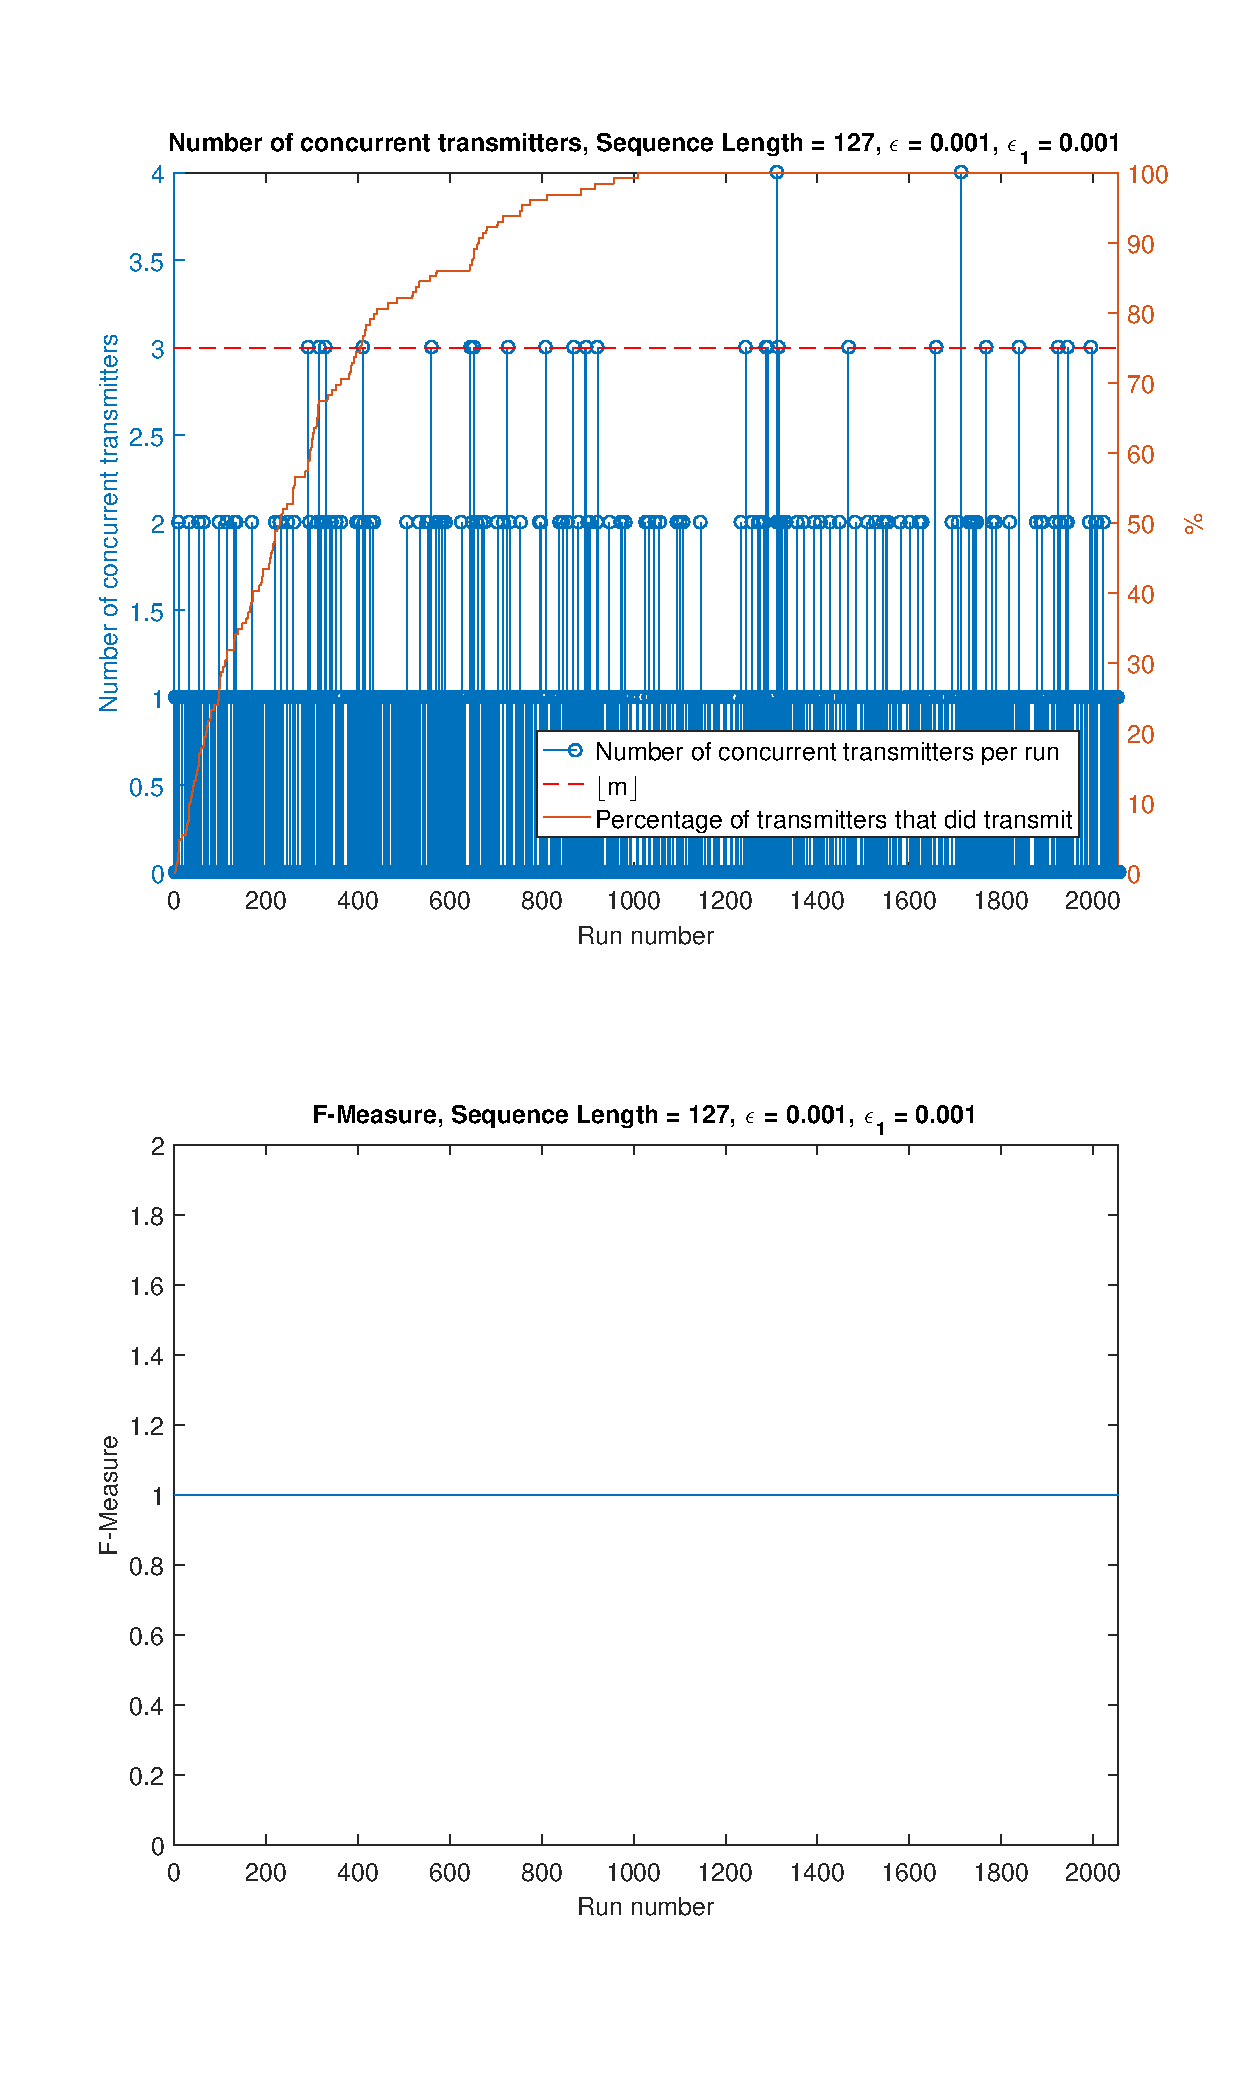
\includegraphics[width=\textwidth]{chapters/evaluation-chapters/simulation/sim-concurrent-tx-and-f-measure-eps=001-n=7.eps}
	\caption{Results of the simulation. Upper plot shows the number of concurrent transmitters per run along with $m$. The lower plot shows the F-measure per run.}
	\label{fig:sim-concurrent-tx-and-f-measure-eps=001-n=7}
\end{figure}

 

These simulations show that for the probabilistic method there is a clear trade off between time and accuracy.
For a given set of sequences, a low value for $\epsilon$ gives high accuracy but the also the a high time.
A high value for $\epsilon$ gives lower accuracy but the also the time becomes smaller.
A low value for $\epsilon_1$ yields a high completeness, in terms of transmitters that have transmitted, for the simulation but also makes the time grow larger.
A simulation with a high value for $\epsilon_1$ will have a low completeness but is also done more quickly.









% CONCLUSIONS AND FUTURE WORK
% !TeX root = ../thesis.tex

\chapter{Conclusions and Future Work}
\label{chp:conclusionsandfuturework}

	\section{Conclusions}


	The aim of this thesis is to find out if lights could be identified as being on or off, by measuring the aggregated energy draw of those lights, with the help of VLC and a single smart-meter.
	CDMA codes have been investigated and compared to see which is the best suited for this scenario.
	Two solutions have been discussed to overcome the interference problem that comes with these types of codes.
	When these codes were understood and made usable in software simulations, two practical testbed were developed, for DC and AC, in order to experiment with.
	When the correct codes are used dependent on the size of the system, each individual light in each testbed could be successfully identified as being on or off in a timely manner.
	For larger systems a simulation was performed which shows that there can be made a trade-off between time and accuracy. 
	But the simulation showed that even with a high accuracy, the lights could still be identified in a timely manner.
	%As the testbed only represents a case where only these lights were connected, there is more work to be done when for instance there are also other appliances connected.






\section{Future Work}


This work is only the first step to disaggregate which lights are on and off.
There remains more work to be done, below there are ideas for future work.

	\subsection{Power Limiting Capacitor}

	The solution of using a capacitor in order to limit the power dissipated in the current source, introduced in \autoref{subsec:ac-modulator} can be further investigated.
	In particular what the drawbacks or benefits are of the of the current that is phase-shifted.
	And if the triggering circuit will still function properly or what the modifications are that need to be made in order for this scheme to work properly.


	\subsection{Other Appliances}

	As the testbeds represent cases where only these lights were connected, the question rises: What will happen when other appliances are connected ?
	These could for example be an incandescent light bulb or a refrigerator.
	To answer that question sample data from \cite{kolter2011redd} could be taken to represent some household appliances and added with the data of the modulation shown from the testbeds.
	Then signal filtering techniques could be performed to try and filter the signal from the modulating lights, given the fact that we know that these lights operate at a certain constant frequency.


	\subsection{Dimming Lights}

	LEDs can be often too bright for a persons liking, so the lights are dimmed.
	Dimming of an LED can be done in two ways: PWM, by lowering the duty cycle and so less power is dissipated by the LED or by limiting the current that flows through the LED.
	Since the LEDs are modulating via an OOK scheme, PWM cannot be used so instead current limiting must be done in order to dim the lights.
	But the CDMA codes are designed to work with each transmitter or LED has the same amplitude or in this case the same current.
	By dimming the LED and changing the current the codes may not work anymore.
	A solution for this can be that each LED will have multiple dimming levels and that for each dimming level other frequencies are used to modulate at.
	A filter can then be used to filter between these LEDs which all have the same amplitude.



	\subsection{Transmitting Data}

	With the current state of this system the LEDs can be identified as being on or off by detecting if their unique code is present or not.
	This can be seen as transmitting data, namely one bit, if the LED is on or off.
	If the LED needs to send other data about the status of the light two approaches can be thought of: 


	\begin{itemize}
		\item The unmodified code assigned to the light will be transmitted for the data-bit `0' and the negation of the code will be transmitted for the data-bit `1'. 
		This gives a problem with the definition of the cross-correlation, which is defined only for the unmodified codes. 
		When the negation of the codes is also used, the cross-correlation between the LEDs that are transmitting is no longer bounded by the mathematical formula and all the calculation on how many LEDs can transmit at the same time can no longer be used with these codes.
		It can be investigated if other codes do have a cross-correlation definition where the negation of the codes is also taken into consideration.

		\item Assign two unique codes from the same set to each light. 
		The lights will send the first code for the data-bit `0' and the second code for the data-bit `1'.
		Since the cross-correlation is defined for the codes from the same set this solution should not yield any problems.
		But further investigation may be required to see if this is a viable solution.
	\end{itemize}


	














% BIBLIOGRAPHY
%#define SORTED 1
\bibliographystyle{bib/latex8}
\bibliography{bib/mycollection}

\appendix


% !TeX root = ../../../thesis.tex

\chapter{DC Testbed Schematic}
\label{app:dc-test-bed-schematic}

\begin{figure}[htb]
	\includegraphics[angle=90,width=\textwidth,height=\textheight,keepaspectratio]{chapters/appendix/dc-test-bed/dc-test-bed-schematic.jpg}
	\caption{Schematic of the DC testbed, to modulate six individual LEDs and measure the combined current.}
	\label{fig:dc-test-bed-schematic}
\end{figure}



% !TeX root = ../../../thesis.tex

\chapter{Modified 230 V AC LED Schematic}
\label{app:commercial-230v-ac-modified-schematic}

In this chapter, the schematic of the original and modified circuit of a commercial 230 V AC LED can be found in \autoref{fig:commercial-230v-ac-modified-schematic}.
The relevant datasheets for parts used, can be found in: \cite{4n35-optocoupler-datasheet}, \cite{mth6n60-n-power-fet-datasheet} and \cite{mje13009g-npn-power-transistor-datasheet}.




\begin{figure}[htb]
	\includegraphics[angle=90,width=\textwidth,height=.9\textheight,keepaspectratio]{chapters/appendix/commercial-230v-ac-modified-schematic/commercial-230v-ac-modified-schematic.jpg}
	\caption{Schematic of the modified commercial 230 V AC LED. Everything in black is from the original schematic. Everything in red is added in order to modulate the LED safely with a micro-controller.}
	\label{fig:commercial-230v-ac-modified-schematic}
\end{figure}


% !TeX root = ../../../thesis.tex

\chapter{Custom LED Modulator Schematic}
\label{app:custom-led-modulator-schematic}

In this chapter, the schematic of the LED modulator can be found in \autoref{fig:custom-led-modulator-schematic}.
The relevant datasheets for parts used, can be found in: \cite{lm7805-vr-datasheet}, \cite{2n7000-n-fet-datasheet}, \cite{sfh617a-optocoupler-datasheet}, \cite{h11l1-optocoupler-datasheet}, \cite{buz80-n-fet-datasheet} and \cite{2n3904-npn-transistor-datasheet}.


\begin{figure}[htb]
	\includegraphics[angle=90,width=\textwidth,height=.9\textheight,keepaspectratio]{chapters/appendix/custom-modulator/custom-modulator-schematic.jpg}
	\caption{Schematic of the LED modulator consisting of a current source with optocoupler, triggering circuit with optocoupler and non-disturbing voltage source.}
	\label{fig:custom-led-modulator-schematic}
\end{figure}


% !TeX root = ../../../thesis.tex

\chapter{Custom Current Sampler Schematic}
\label{app:custom-current-sampler-schematic}

In this chapter, the schematic of the current-sampler used to measure the current of the 230 V AC can be found in \autoref{fig:custom-current-sampler-schematic}.
The relevant datasheets for parts used, can be found in: \cite{lm7824-vr-datasheet}, \cite{lm7805-vr-datasheet}, \cite{lm336z-ref-voltage-datasheet}, \cite{mcp3204-adc-datasheet}, \cite{iso7241m-spi-isolator-datasheet}, \cite{2n7000-n-fet-datasheet} and \cite{sfh617a-optocoupler-datasheet}.


\begin{figure}[htb]
	\includegraphics[angle=90,width=\textwidth,height=.9\textheight,keepaspectratio]{chapters/appendix/custom-current-sampler/custom-current-sampler-schematic.jpg}
	\caption{Schematic of the current sampler, with an external ADC which is isolated from the micro-controller and with a triggering circuit.}
	\label{fig:custom-current-sampler-schematic}
\end{figure}








\end{document}

